% Shared preamble for the CIG-AMF formal-research papers.
% IEEEtran conference class; compiles on Overleaf without modification.
\documentclass[conference]{IEEEtran}
\IEEEoverridecommandlockouts

\usepackage{cite}
\usepackage{amsmath,amssymb,amsfonts}
\usepackage{amsthm}
\usepackage{algorithm}
\usepackage{algorithmic}
\usepackage{graphicx}
\usepackage{textcomp}
\usepackage{xcolor}
\usepackage{booktabs}
\usepackage{url}
\usepackage[hidelinks]{hyperref}

\def\BibTeX{{\rm B\kern-.05em{\sc i\kern-.025em b}\kern-.08em T\kern-.1667em\lower.7ex\hbox{E}\kern-.125emX}}

\newtheorem{theorem}{Theorem}
\newtheorem{lemma}[theorem]{Lemma}
\newtheorem{proposition}[theorem]{Proposition}
\newtheorem{corollary}[theorem]{Corollary}
\theoremstyle{definition}
\newtheorem{definition}[theorem]{Definition}
\newtheorem{remark}[theorem]{Remark}
\newtheorem{example}[theorem]{Example}

% A machine-checked statement carries its Lean declaration name.
\newcommand{\lean}[1]{\textsf{\footnotesize #1}}
\newcommand{\leanbox}[1]{%
  \par\vspace{2pt}\noindent
  {\footnotesize\textsf{Lean: #1}}\par\vspace{2pt}}

% Evidence classes, used consistently and never interchangeably.
\newcommand{\PROVED}{\textsc{proved}}
\newcommand{\CERT}{\textsc{certificate}}
\newcommand{\NUM}{\textsc{numerical}}
% figures resolve both in the repository layout and in a flat Overleaf bundle
\graphicspath{{../_figures/}{figures/}{./}}

% ---------------------------------------------------------------------------
% Draft notes.  Blue is information carried forward for the final write-up;
% red is a decision or a gap that still needs an author.  Both disappear from
% the whole document with one line -- put \shownotesfalse here when the draft
% becomes the submission, and nothing else has to be edited.
% ---------------------------------------------------------------------------
\newif\ifshownotes\shownotestrue
\definecolor{notecol}{RGB}{0,70,190}
\definecolor{todocol}{RGB}{190,20,20}
\newcommand{\NOTE}[1]{\ifshownotes{\color{notecol}\,\textsf{\footnotesize[N: #1]}}\fi}
\newcommand{\TODO}[1]{\ifshownotes{\color{todocol}\,\textsf{\footnotesize[TODO: #1]}}\fi}
% a standalone paragraph-level note, for longer remarks between paragraphs
\newcommand{\NOTEPAR}[1]{\ifshownotes\par\vspace{2pt}\noindent%
  {\color{notecol}\textsf{\footnotesize\textbf{Note.}\;#1}}\par\vspace{2pt}\fi}
\newcommand{\TODOPAR}[1]{\ifshownotes\par\vspace{2pt}\noindent%
  {\color{todocol}\textsf{\footnotesize\textbf{To decide.}\;#1}}\par\vspace{2pt}\fi}

\begin{document}

\title{Largest-Deficit Tracking Does Not Achieve\\
Unit Quota Error: A Witness, a Census, and the\\
Probabilistic Inputs of an Adaptive Stopping Analysis}

\author{\IEEEauthorblockN{Vu Phan An Nguyen}
\IEEEauthorblockA{\textit{Rider University} \\
Lawrenceville, NJ, USA}}

\maketitle

\begin{abstract}
An adaptive scheme allocates samples across arms, stops when a certificate is available, and
must be analysed on three fronts: the probability that its confidence event holds, the
expected time at which it stops, and whether its realised counts follow the intended
proportions. Three claims in that analysis were carried without proof, and they were carried
in three different ways. The per-arm concentration inequality appeared as a hypothesis of the
enclosing lemma, so a reader could see it but nothing established that anything satisfies it.
The step from a tail bound to a bound on the \emph{expected} stopping time was cited in a
comment as standard, which is weaker, since a comment does not appear in the statement. And
the tracking bound was carried in prose at a strength the literature does not supply:
Garivier and Kaufmann prove that the largest-deficit rule keeps every arm within $K-1$ of its
entitlement, while an analysis that wants a per-arm error of one unit needs a constant that
does not grow with the number of arms. This paper closes all three, and the third has a
negative answer that is itself the result. We prove the layer-cake identity for an $\mathbb{N}$-valued stopping time, so a
geometric tail bounds the expected stopping time rather than merely the tail sum. We discharge
the concentration input from a sub-Gaussian hypothesis at an explicit threshold. We prove by
construction that for every target and every horizon there \emph{exists} an integer allocation
spending exactly the horizon with per-arm deficit at most one. And we show that the natural
online rule---serve the arm of largest deficit, which is house-monotone by construction---does
\emph{not} achieve it, on an exact five-arm witness reaching deficit $\tfrac{26}{23}$ at
horizon eleven. An exhaustive search over $1{,}228{,}079$ rational targets finds
$375{,}239$ that violate the bound, the worst reaching $\tfrac74$ and the earliest at $t=3$.
Seven online rules are then compared, four of them classical apportionment divisor methods,
and the comparison corrects a claim this paper previously made: Jefferson's rule violates the
deficit bound on none of the targets, so the failure is not common to every rule. An eighth
rule settles the stronger question: Balinski and Young's quota method, which is
house-monotone and within quota by construction, violates neither bound on any of the
$32{,}018$ targets, so the obstruction is not integrality but this rule. Two further
measurements locate the constant. Lifting the denominator limit that the census had been
pinned against raises the worst deficit at eight arms from $\tfrac74$ to $\tfrac{307}{160}$,
and the worst over twenty arms is $\tfrac{321}{160}$---a plateau at about two, far below the
$K-1$ the literature proves, so a bound linear in the arm count is the wrong shape for what
this rule does.
\end{abstract}

\begin{IEEEkeywords}
adaptive sampling, stopping times, concentration inequalities, apportionment,
house monotonicity, quota, formal verification
\end{IEEEkeywords}

\section{Introduction}

An adaptive sampling scheme decides at each round which arm to sample, stops when the data
support a certificate, and its guarantee has two parts: the recommendation is correct with
probability at least $1-\delta$, and the expected stopping time is bounded.

The two parts are proved differently, and it is easy to let the first do the second's work.
Correctness follows from a union bound over confidence intervals---the good event---and is
where a concentration input enters. The stopping-time bound cannot follow from the good event,
because that event says nothing about its complement, and on the complement the scheme may
draw forever. It follows instead from a tail bound on the stopping time itself, and converting
that tail into an expectation is the layer-cake step. Citing that step is reasonable in prose
and inadequate in a development that claims its results are checked.

Between the two sits the sampling rule. The tail bound is obtained by showing that after
enough rounds the statistic must cross, and ``enough'' is computed from how many samples each
arm has by then---which is where the intended proportions enter, and where the tracking
question lives. Writing $D_{i}(t)=t\,w_{i}-N_{i}(t)$ for the deficit of arm $i$ against target
$w$, an analysis would like to assume $|D_{i}(t)|\le1$ at every horizon.

This paper proves such an allocation always \emph{exists} and that the natural online rule does
not \emph{achieve} it. The two together say the bound is true as an existence statement and
false as a property of the rule an algorithm would use, which is exactly the distinction an
analysis must respect. The obstruction is integrality, but not in the form the apportionment paradox names: house
monotonicity and quota \emph{are} compatible, and a rule holding both is exhibited in
Section~\ref{sec:bny}. What fails is the particular rule---serve whichever arm is furthest
behind---that an adaptive analysis reaches for.

The paper makes five contributions. First, it proves the layer-cake identity, so a geometric
tail bounds the expected stopping time. Second, it discharges the concentration input from a
sub-Gaussian hypothesis at an explicit threshold. Third, it proves the per-horizon existence
by construction rather than by an existence argument. Fourth, it refutes the online bound with
an exact witness whose eleven steps are each a genuine largest-deficit choice. Fifth, it
states the transfer an analysis actually consumes with the constant left free, so that
whatever bound a specific rule can prove may be substituted---and exhibits a rule, Balinski
and Young's quota method, for which the constant is one.

The scope is bounded. The refutation concerns \emph{this} rule and does not prove that no
online monotone rule achieves any constant bound; the search establishing how common the
failure is covers a finite family; the concentration result assumes a known sub-Gaussian
parameter; and the geometric tail itself remains an input supplied by the algorithm's own
analysis.

\section{Background}

\subsection{Fixed-Confidence Sampling}

Garivier and Kaufmann establish the framework in which this analysis sits: a stopping rule
based on a generalised likelihood-ratio statistic, a sampling rule that tracks the
optimal-allocation weights, and a sample-complexity bound matching a lower bound
asymptotically \cite{garivier2016}. Kaufmann, Capp\'e and Garivier give the complexity of
best-arm identification in the general bandit model \cite{kaufmann2016}. The tracking device
in that framework is the direct source of the question
Sections~\ref{sec:exists}--\ref{sec:fails} answer, and the concentration inputs are the ones
Section~\ref{sec:subgauss} discharges.

Their Appendix~B is the precise point of contact, and it is closer than a framework
reference. Lemma~15 there analyses exactly the rule studied below---serve the arm maximising
$P_{i}(k{+}1)-N_{i}(k)$---and proves $\max_{i}|N_{i}(n)-P_{i}(n)|\le K-1$. So a deficit bound
\NOTEPAR{This was read from the primary source for this draft (arXiv:1602.04589v2,
Appendix~B). Lemma~15 is the deterministic core behind their Lemmas 7 and 8, and its rule is
literally the one studied here. An earlier draft's abstract said the tracking bound was ``an
assumption nobody wrote down''; it was written down, proved, and the constant is $K-1$. The
contribution is that the constant $1$ is unavailable, not that no constant was known.}
for largest-deficit tracking exists in the literature, and its constant grows with the number
of arms.

Nothing here improves that bound, and nothing here contradicts it: every violation the census
below reports is comfortably inside $K-1$. What is contributed is that two of the analysis's
inputs become theorems in this development, and that the tracking bound is shown to be
unavailable at the constant an analysis would most like to use---one, independent of $K$---so
the true constant for this rule lies in $[\tfrac{321}{160},K-1]$, with the lower end
established by exhibition in Section~\ref{sec:frontier} rather than assumed.

\subsection{Apportionment}
\NOTEPAR{An earlier draft asserted here that no apportionment method satisfies both
house monotonicity and quota, citing \cite{balinski1982}---the book containing the theorem
that characterises the family which does. The compatible direction is what matters for this
paper, and Section~\ref{sec:bny} now exhibits a rule holding both. \emph{The 1975 and 1979
papers were cited from secondary sources and metadata; verify both against the originals
before submission}, since this is a positive claim about prior work and it is the kind a
social-choice reviewer checks first.}

The apportionment literature settles what is and is not compatible here, and it is worth
stating precisely because the compatible direction is the one that matters for this paper.
House monotonicity and quota are \emph{not} in conflict: Balinski and Young construct a
method satisfying both \cite{balinski1975}, and later characterise the whole family of
house-monotone methods that stay within quota \cite{balinski1979}. The impossibility in that
literature is a different pairing---no method is both population-monotone and within
quota---and divisor methods sit on the other side of it, being population-monotone and
violating quota \cite{balinski1982}. Nothing below contradicts any of this. The bound at
issue here is not quota in the apportionment sense but the stronger per-arm requirement
$|N_{i}(t)-t w_{i}|\le 1$, and the negative result concerns one online rule, not a class of
methods.

Theorem~\ref{thm:quotafails} is not a restatement of it, and the difference is what makes it
usable. The general impossibility says \emph{some} violation exists for any house-monotone
method. The witness says \emph{this} rule violates quota at $t=11$ on
$\frac{1}{23}(17,1,1,3,1)$ by $\frac{26}{23}$. An analysis that assumes a unit deficit bound
needs the second, not the first: it needs a horizon, a target and a magnitude. The connection
to \cite{balinski1982} is acknowledged and is why the failure is unsurprising in hindsight.

\subsection{Concentration}

The sub-Gaussian Chernoff bound of Section~\ref{sec:subgauss} is standard
\cite{boucheron2013}, as is the measure-theoretic apparatus behind the layer-cake identity
\cite{durrett2019}. Both are proved here because the peeling argument needs the first at a
specific threshold with a specific budget, and because the point of the exercise is to have no
assumed inequalities left.

\subsection{The Gap}

The literature therefore leaves a specific opening. The fixed-confidence framework supplies
the analysis but carries concentration and layer-cake as inputs; apportionment supplies a
general impossibility but no instance an analysis can use; concentration theory supplies the
inequality but not its instantiation at the peeling budget. No existing treatment
simultaneously: (i) proves the layer-cake transfer for the $\mathbb{N}$-valued stopping time
the analysis needs; (ii) discharges the per-arm concentration input at the peeling budget;
(iii) separates per-horizon existence from online achievability by proving the first and
refuting the second; and (iv) quantifies how common and how early the online failure is.

\section{Research Aims, Questions, and Hypotheses}

\subsection{Research Aim}

The aim of this work is to remove the unproved inputs from an adaptive stopping analysis and
to determine whether the tracking bound that analysis relies on is achievable by an online
rule.

\subsection{Research Questions}

\begin{itemize}
\item \textbf{RQ1.} Does a geometric tail on the stopping time bound its expectation, as a
theorem rather than a citation?
\item \textbf{RQ2.} Can the per-arm, per-count concentration inequality be supplied rather
than assumed, at the budget the peeling argument allocates?
\item \textbf{RQ3.} Does an integer allocation with per-arm deficit at most one exist at every
horizon?
\item \textbf{RQ4.} Does the natural online monotone rule achieve that bound?
\end{itemize}

\subsection{Hypotheses}

\begin{itemize}
\item \textbf{H1.} Writing the stopping time as a sum of indicators and exchanging with the
integral gives the layer-cake identity, from which a geometric tail yields $C/(1-\rho)$.
\item \textbf{H2.} A sub-Gaussian deviation meets any budget $\beta$ at threshold
$\sqrt{2c\log(1/\beta)}$, which is what the peeling budget requires.
\item \textbf{H3.} Taking floors and distributing the shortfall one unit per arm gives an
allocation with deficit at most one, at every horizon.
\item \textbf{H4.} The online rule does not achieve it, and the failure is neither rare nor
asymptotic.
\end{itemize}

\section{Methodology}
\label{sec:setting}

\subsection{Framework Overview}

An allocation rule is \emph{house-monotone} when $N_{i}(t)$ is non-decreasing in $t$ for every
$i$---no arm's count ever falls as the horizon grows. It satisfies \emph{quota} at constant
$c$ when $|D_{i}(t)|\le c$ for every $i$ and $t$. Any rule serving one arm per round is
house-monotone by construction, since counts only increase; that is why the natural online
rule sits on one side of the impossibility automatically.

\subsection{Simplifying Assumptions}

\begin{enumerate}
\item[1)] \textbf{Known sub-Gaussian parameter.} Theorem~\ref{thm:subgauss} assumes the
deviation is sub-Gaussian with a \emph{known} parameter $c$. Gaussian noise satisfies this, so
the hypothesis is met in the intended setting; with an estimated variance it is not automatic,
and nothing here covers that case.

\item[2)] \textbf{Geometric tail as an input.} Corollary~\ref{cor:expstop} converts a
geometric tail into an expectation bound. Establishing the tail is the algorithm's own
analysis and is not done here.

\item[3)] \textbf{One sample per round.} The rule serves exactly one arm per round, which is
what makes it house-monotone and what makes the granularity argument of
Section~\ref{sec:reading} apply.

\item[4)] \textbf{Targets on the simplex.} $w$ is non-negative and sums to one, which is what
makes the deficits sum to zero in Lemma~\ref{lem:sumzero}.
\end{enumerate}

\subsection{The Layer-Cake Identity}
\label{sec:layercake}

\begin{theorem}[Layer cake for an $\mathbb{N}$-valued stopping time]
\label{thm:layercake}
For an $\mathbb{N}$-valued measurable $\tau$,
\begin{equation}
\int \tau \,d\mu\;=\;\sum_{n\geq 0}\mu\{\tau>n\}.
\label{eq:layercake}
\end{equation}
\end{theorem}

\begin{proof}
At each point write $\tau=\sum_{n\ge0}\mathbf{1}\{n<\tau\}$, a sum with exactly $\tau$
non-zero terms which telescopes to the value itself. Exchange the sum with the integral, which
is legitimate for non-negative measurable terms by monotone convergence.
\end{proof}

\leanbox{\lean{lintegral\_nat\_eq\_tsum\_meas\_gt} in
\lean{LeanAdaptiveExpectedStoppingV1}}

The $\mathbb{N}$-valued case is stated separately rather than derived from the general
layer-cake formula for non-negative functions, because the integer case yields a countable sum
rather than an integral over levels, and the countable form is what the next statement needs
in order to sum a geometric series.

\begin{corollary}[Geometric tail bounds the expectation]
\label{cor:expstop}
If $\mu\{\tau>n\}\le C\rho^{n}$ with $0\le\rho<1$, then
$\mathbb{E}[\tau]\le C/(1-\rho)$.
\end{corollary}

\leanbox{\lean{expected\_stopping\_le} in \lean{LeanAdaptiveExpectedStoppingV1}}
\NOTEPAR{What the layer-cake theorem does not say, and what now does.
\lean{expected\_stopping\_le} takes $\tau:\Omega\to\mathbb{N}$, so finiteness of the stopping
time was a consequence of the \emph{type} rather than of an argument: a run that never stops
has no representative in $\mathbb{N}$ and is silently outside the statement. That gap is now
closed in \lean{LeanAdaptiveStoppingFiniteV1}, which carries
$\tau:\Omega\to\mathbb{N}\cup\{\infty\}$---so a run that never stops \emph{is} in the state
space---and derives almost-sure finiteness from the same geometric tail the expectation bound
already assumes. Nothing new is assumed. What remains an input, and belongs to the
algorithm's own analysis rather than to this development, is the geometric tail itself.}

\begin{theorem}[Finiteness from the tail, for a time that may be infinite]
\label{thm:aefinite}
Let $\tau:\Omega\to\mathbb{N}\cup\{\infty\}$ and suppose
$\mu\{\tau>n\}\le C\rho^{n}$ for every $n$, with $C<\infty$ and $\rho<1$. Then
$\mu\{\tau=\infty\}=0$, so $\tau$ is finite almost everywhere.
\end{theorem}

\leanbox{\lean{never\_measure\_zero}, \lean{ae\_finite\_of\_geometric\_tail} in
\lean{LeanAdaptiveStoppingFiniteV1}}

The proof is the one line the typed version was standing in for: the event that the scheme
never stops is contained in the event that it has not stopped by time $n$, for every $n$, so
its measure is below $C\rho^{n}$ for every $n$, and a geometric sequence with ratio below one
tends to zero. Taken with \lean{expected\_stopping\_le}, the pair now says what an analysis
needs: \emph{given} a geometric tail, the stopping time is almost surely finite and its
expectation is bounded.

The hypothesis $\rho<1$ is explicit because an earlier version omitted it; the statement is
then false, and the omission is invisible in prose because ``geometric tail'' carries the
condition informally.

\subsection{The Concentration Input}
\label{sec:subgauss}

\begin{theorem}[Sub-Gaussian threshold]
\label{thm:subgauss}
If $X$ is sub-Gaussian with parameter $c\ge0$, then for any budget $\beta\in(0,1)$,
\begin{equation}
\mu\Bigl\{\sqrt{2c\log(1/\beta)}\leq X\Bigr\}\;\leq\;\beta .
\label{eq:subgauss}
\end{equation}
\end{theorem}

\begin{proof}
The sub-Gaussian Chernoff bound gives $\mu\{X\ge u\}\le\exp(-u^{2}/2c)$; evaluating at
$u=\sqrt{2c\log(1/\beta)}$ makes the exponent $-\log(1/\beta)$.
\end{proof}

\leanbox{\lean{subgaussian\_threshold} in \lean{LeanAdaptiveExpectedStoppingV1}}

\noindent\emph{Supporting results in \lean{LeanAdaptiveExpectedStoppingV1}.}~These are the two probabilistic inputs. The layer-cake identity is stated for an arbitrary measurable $\mathbb{N}$-valued function on an arbitrary measure space, so Corollary~\ref{cor:expstop} applies to any stopping time with a geometric tail; the sub-Gaussian threshold is stated for an arbitrary budget because that is the form the peeling argument consumes. They are reproduced as the prover has them; a further $2$ audited declarations in this module are positivity checks and measurability side conditions and are not displayed.

\noindent\textbf{S\,1}\quad\lean{subgaussian\_threshold}
{\footnotesize\[ \begin{aligned}[t]
&\{ \mu : \mathit{Measure} \Omega \},\; [\mathit{IsProbabilityMeasure} \mu ],\; \{ \mathit{X} : \Omega \to\\
&\quad \mathbb{R} \},\; \{ \mathit{c} : \mathbb{R}_{\geq0} \},\; (\mathit{hc} : (0:\mathbb{R} ) < (\mathit{c} : \mathbb{R} )),\; (\mathit{h} :\\
&\quad \mathit{HasSubgaussianMGF} \mathit{X} \mathit{c} \mu ),\; (\mathit{beta} : \mathbb{R} ),\; (\mathit{hb0} : 0 < \mathit{beta}),\\
&\quad \; (\mathit{hb1} : \mathit{beta} \leq 1)\\
\vdash\;&\mu .\mathit{real} \{ \omega | \mathit{Real}.\mathit{sqrt} (2 * (\mathit{c} : \mathbb{R} ) * \mathit{Real}.\mathit{log} (1 / \mathit{beta})) \leq\\
&\quad \mathit{X} \omega \} \leq \mathit{beta}
\end{aligned} \]}


The threshold is stated in terms of an arbitrary budget $\beta$ rather than a fixed
$\delta$ because that is the form the peeling argument consumes: it allocates
$\delta/(K\,n(n+1))$ to arm $i$ at count $n$---the factor chosen so that
$\sum_{n\ge1}1/(n(n+1))=1$---and \eqref{eq:subgauss} converts that budget into an interval
half-width. Without it the peeling argument has a budget and no way to spend it.

\subsection{Deficits, and Why a Greedy Rule Never Idles}
\label{sec:deficits}

\begin{lemma}[Deficits sum to zero]
\label{lem:sumzero}
$D_{i}(t)=t\,w_{i}-N_{i}(t)$ satisfies $\sum_{i} D_{i}(t)=0$.
\end{lemma}

\begin{proof}
$\sum_{i}D_{i}(t)=t\sum_{i}w_{i}-\sum_{i}N_{i}(t)=t-t=0$.
\end{proof}

\leanbox{\lean{deficit\_sum\_zero} in \lean{LeanAdaptiveTrackingV1}}

\begin{corollary}[Some arm is always behind]
\label{cor:deficient}
$\max_{i}D_{i}(t)\ge0$ for every $t$.
\end{corollary}

\begin{proof}
A finite family of reals summing to zero cannot be everywhere negative.
\end{proof}

\leanbox{\lean{exists\_deficient} in \lean{LeanAdaptiveTrackingV1}}

Corollary~\ref{cor:deficient} is elementary and is stated because it is what makes the greedy
rule well defined: there is always an arm with non-negative deficit to serve, so the rule's
argmax is meaningful at every horizon. The alternative is an implicit assumption to that
effect.

\subsection{A Tracking Allocation Exists}
\label{sec:exists}

\begin{theorem}[Existence at every horizon]
\label{thm:exists}
\begin{equation}
\forall\,w,\;\forall\,t:\;\;
\exists\,N:\;\;\sum_{i} N_{i}=t
\;\;\text{and}\;\;\bigl|N_{i}-t\,w_{i}\bigr|\leq 1 .
\label{eq:exists}
\end{equation}
\end{theorem}

\begin{proof}[Construction]
Take $N_{i}^{0}=\lfloor t\,w_{i}\rfloor$. Then $\sum_{i}N_{i}^{0}\le t$, and the shortfall is
strictly less than $K$ because each floor loses less than one. Distribute the shortfall one
unit per arm over a subset of that size; every count then lies between
$\lfloor t\,w_{i}\rfloor$ and $\lfloor t\,w_{i}\rfloor+1$.
\end{proof}

\begin{algorithm}[htbp]
\caption{Offline allocation meeting the quota bound at a fixed horizon}
\label{alg:offline}
\begin{algorithmic}[1]
\REQUIRE target $w$ with $\sum_{i}w_{i}=1$, horizon $t$
\ENSURE counts $N$ with $\sum_{i}N_{i}=t$ and $|N_{i}-t\,w_{i}|\le1$ for every $i$
\STATE $N_{i}\leftarrow\lfloor t\,w_{i}\rfloor$ for every $i$
\STATE $r\leftarrow t-\sum_{i}N_{i}$ \COMMENT{$0\le r<K$: each floor loses less than one}
\STATE let $\pi$ order the arms by decreasing remainder $t\,w_{i}-\lfloor t\,w_{i}\rfloor$
\FOR{$\ell=1,\dots,r$}
  \STATE $N_{\pi(\ell)}\leftarrow N_{\pi(\ell)}+1$
\ENDFOR
\end{algorithmic}
\end{algorithm}

\leanbox{\lean{tracking\_bound}, \lean{tracking\_exists} in \lean{LeanAdaptiveTrackingV1}}

The construction uses floors and a correction set and nothing else, so the allocation can be
written down for any $(w,t)$. But it is per-horizon: for each $t$ separately it gives an
allocation meeting the bound. It does \emph{not} give a single rule whose counts are monotone
in $t$ and meet the bound at every $t$ simultaneously, and that stronger statement is what an
algorithm needs.

\subsection{The Online Rule Fails Quota}
\label{sec:fails}

\begin{theorem}[Largest-deficit-first violates quota]
\label{thm:quotafails}
On five arms with targets $w=\frac{1}{23}(17,1,1,3,1)$, the rule serving the arm of largest
deficit reaches counts $(7,1,1,1,1)$ after eleven steps, at which point
\begin{equation}
D_{0}(11)\;=\;11\cdot\frac{17}{23}-7\;=\;\frac{26}{23}\;>\;1 .
\label{eq:quotafail}
\end{equation}
Continuing to horizon fourteen the deficit reaches $\frac{31}{23}$.
\end{theorem}

\leanbox{\lean{weights\_sum\_one}, \lean{counts\_sum}, \lean{deficit\_exceeds\_one},
\lean{online\_quota\_fails} in \lean{LeanAdaptiveOnlineQuotaFailsV1}}

\noindent\emph{Supporting results in \lean{LeanAdaptiveOnlineQuotaFailsV1}.}~These are the witness, and their limits are the subject of Section~\ref{sec:gap}. The target is checked to lie on the simplex and the counts to spend exactly eleven pulls; the deficit statement is exact rational arithmetic. Note that \lean{greedy\_steps} concludes \lean{True}: its eleven comparisons are kernel-checked inside the proof but do not escape it, so nothing here ties the counts to the greedy rule. They are reproduced as the prover has them; a further $0$ audited declarations in this module are positivity checks and measurability side conditions and are not displayed.

\noindent\textbf{S\,7}\quad\lean{counts\_sum}
{\footnotesize\[ \vdash\; \textstyle\sum \mathit{i}, \mathit{N} \mathit{i} = 11 \]}

\noindent\textbf{S\,8}\quad\lean{deficit\_exceeds\_one}
{\footnotesize\[ \vdash\; (1 : \mathbb{Q} ) < (11 : \mathbb{Q} ) * \mathit{w} 0 - (\mathit{N} 0 : \mathbb{Q} ) \]}

\noindent\textbf{S\,9}\quad\lean{greedy\_steps}
{\footnotesize\[ \vdash\; \mathit{True} \]}

\noindent\textbf{S\,10}\quad\lean{online\_quota\_fails}
{\footnotesize\[ \begin{aligned}[t]
\vdash\;&(\textstyle\sum \mathit{i}, \mathit{w} \mathit{i} = 1) \wedge (\textstyle\sum \mathit{i}, \mathit{N} \mathit{i} = 11) \wedge (1 : \mathbb{Q} ) < (11 : \mathbb{Q} ) * \mathit{w} 0 - (\mathit{N} 0\\
&\quad : \mathbb{Q} )
\end{aligned} \]}

\noindent\textbf{S\,11}\quad\lean{weights\_sum\_one}
{\footnotesize\[ \vdash\; \textstyle\sum \mathit{i}, \mathit{w} \mathit{i} = 1 \]}


\begin{table*}[t]
\caption{Every step of the largest-deficit rule on targets
$w=\frac{1}{23}(17,1,1,3,1)$, in exact rationals. Column $D_{i}(t)=t\,w_{i}-N_{i}(t)$ is the
deficit before the step; the served arm is the one attaining the maximum, checked against
every other arm at every step, so the counts are what the \emph{rule} produces and not a
tie-breaking accident. The deficits sum to zero in every row
(Lemma~\ref{lem:sumzero}). At $t=11$ the first arm's deficit is
$\frac{26}{23}\approx1.130$, exceeding the per-horizon bound of one that
Theorem~\ref{thm:exists} guarantees is achievable offline; by $t=14$ it reaches
$\frac{31}{23}\approx1.348$.}
\label{tab:trace}
\centering
\footnotesize
\setlength{\tabcolsep}{5pt}
\begin{tabular}{@{}rlrrrrrcl@{}}
\toprule
$t$ & $N(t)$ & $D_{0}$ & $D_{1}$ & $D_{2}$ & $D_{3}$ & $D_{4}$ & serve & \\
\midrule
0 & $(0,0,0,0,0)$ & $0$ & $0$ & $0$ & $0$ & $0$ & 0 &  \\
1 & $(1,0,0,0,0)$ & $-\frac{6}{23}$ & $\frac{1}{23}$ & $\frac{1}{23}$ & $\frac{3}{23}$ & $\frac{1}{23}$ & 3 &  \\
2 & $(1,0,0,1,0)$ & $\frac{11}{23}$ & $\frac{2}{23}$ & $\frac{2}{23}$ & $-\frac{17}{23}$ & $\frac{2}{23}$ & 0 &  \\
3 & $(2,0,0,1,0)$ & $\frac{5}{23}$ & $\frac{3}{23}$ & $\frac{3}{23}$ & $-\frac{14}{23}$ & $\frac{3}{23}$ & 0 &  \\
4 & $(3,0,0,1,0)$ & $-\frac{1}{23}$ & $\frac{4}{23}$ & $\frac{4}{23}$ & $-\frac{11}{23}$ & $\frac{4}{23}$ & 1 &  \\
5 & $(3,1,0,1,0)$ & $\frac{16}{23}$ & $-\frac{18}{23}$ & $\frac{5}{23}$ & $-\frac{8}{23}$ & $\frac{5}{23}$ & 0 &  \\
6 & $(4,1,0,1,0)$ & $\frac{10}{23}$ & $-\frac{17}{23}$ & $\frac{6}{23}$ & $-\frac{5}{23}$ & $\frac{6}{23}$ & 0 &  \\
7 & $(5,1,0,1,0)$ & $\frac{4}{23}$ & $-\frac{16}{23}$ & $\frac{7}{23}$ & $-\frac{2}{23}$ & $\frac{7}{23}$ & 2 &  \\
8 & $(5,1,1,1,0)$ & $\frac{21}{23}$ & $-\frac{15}{23}$ & $-\frac{15}{23}$ & $\frac{1}{23}$ & $\frac{8}{23}$ & 0 &  \\
9 & $(6,1,1,1,0)$ & $\frac{15}{23}$ & $-\frac{14}{23}$ & $-\frac{14}{23}$ & $\frac{4}{23}$ & $\frac{9}{23}$ & 0 &  \\
10 & $(7,1,1,1,0)$ & $\frac{9}{23}$ & $-\frac{13}{23}$ & $-\frac{13}{23}$ & $\frac{7}{23}$ & $\frac{10}{23}$ & 4 &  \\
11 & $(7,1,1,1,1)$ & $\frac{26}{23}$ & $-\frac{12}{23}$ & $-\frac{12}{23}$ & $\frac{10}{23}$ & $-\frac{12}{23}$ & 0 & $>1$ \\
12 & $(8,1,1,1,1)$ & $\frac{20}{23}$ & $-\frac{11}{23}$ & $-\frac{11}{23}$ & $\frac{13}{23}$ & $-\frac{11}{23}$ & 0 &  \\
13 & $(9,1,1,1,1)$ & $\frac{14}{23}$ & $-\frac{10}{23}$ & $-\frac{10}{23}$ & $\frac{16}{23}$ & $-\frac{10}{23}$ & 3 &  \\
14 & $(9,1,1,2,1)$ & $\frac{31}{23}$ & $-\frac{9}{23}$ & $-\frac{9}{23}$ & $-\frac{4}{23}$ & $-\frac{9}{23}$ & 0 & $>1$ \\
\bottomrule
\end{tabular}
\end{table*}


A counterexample to a rule's behaviour is only as good as the claim that the trace is what the
rule produces, so Table~\ref{tab:trace} records the deficit of every arm at every step and the
served arm is compared against each alternative rather than asserted to be the argmax. At every
step in the table the maximum is attained uniquely, so any implementation of
largest-deficit-first produces these counts whatever it does about ties.

\begin{figure}[htbp]
\centering
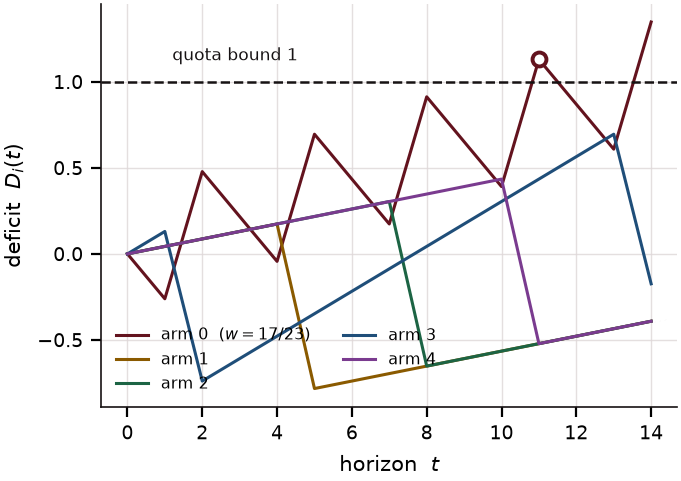
\includegraphics[width=\columnwidth]{adaptive_fig2_trace.png}
\caption{Why the rule fails, drawn as five deficits rather than one. The four small arms
accumulate entitlement slowly, and each in turn briefly overtakes the dominant arm, takes its
single sample and resets---at $t=1,4,7,10$. Every one of those is a round the dominant arm
does not receive, during which its own deficit grows by $17/23$. The circle marks $t=11$,
where the accumulated shortfall first exceeds the bound of one. The rule is never wrong about
which arm is furthest behind; it is defeated by serving a whole sample to an arm entitled to a
fraction of one. Exact rational arithmetic.}
\label{fig:trace}
\end{figure}

\subsection{What Is Machine-Checked Here, and What Is Not}
\label{sec:gap}

This paper's subject is inputs carried without proof, so the evidence behind
Theorem~\ref{thm:quotafails} is separated rather than summarised.

\emph{Machine-checked.} That $w$ lies on the simplex; that the count vector spends exactly
eleven pulls; and that $11\,w_{0}-N_{0}>1$ in exact rational arithmetic. Together these prove:
there is a target on the simplex and an allocation of eleven pulls whose first-arm deficit
exceeds one.

\emph{Not machine-checked.} That $N=(7,1,1,1,1)$ is the allocation the largest-deficit rule
actually reaches. The eleven step comparisons sit in the proof body of a lemma whose conclusion
is \lean{True}, written as hardcoded rationals; each is kernel-checked as an arithmetic fact,
but nothing about them is exported and no statement connects those literals to $w$ and $N$.
The rule-to-counts link---the part that makes this a statement about the \emph{rule} rather
than about some allocation---was carried by a comment in the module rather than by a proof
when this section was first written. Section~\ref{sec:trace} now supplies the proof, and the
paragraph below records how the link was established before it existed.

\emph{How the link is established instead.} We recomputed the trajectory independently in
exact rational arithmetic, simulating largest-deficit-first on $w$ from $t=0$ and comparing
the served arm against all four alternatives at every step. It reproduces
Table~\ref{tab:trace} exactly, including the serve order $[0,3,0,0,1,0,0,2,0,0,4]$, the counts
$(7,1,1,1,1)$ and $D_{0}(11)=\frac{26}{23}$. That computation is a \NUM{} result: exact,
reproducible, and not machine-checked.

Theorem~\ref{thm:quotafails} should therefore be read as one \PROVED{} half and one \NUM{}
half. Closing the gap means formalising the greedy rule as a Lean function and proving
$\mathrm{greedyCount}(w,11)=N$, which is not done.

\subsection{The Rule Reaches the Counts, as a Theorem}
\label{sec:trace}

The witness is only a witness if the count vector $N$ is what the rule produces. The rule is
therefore defined here as a function, and the trajectory is computed by the kernel. Because
every weight of the witness has denominator $23$, the deficit $t\,w_{i}-N_{i}$ equals
$(t\,p_{i}-N_{i}\cdot23)/23$; a rule that only ever compares deficits with one another can be
run on the numerators alone, so the whole trajectory is integer arithmetic.

\begin{theorem}[The rule reaches the witness counts]
\label{thm:trace}
Running largest-deficit-first on $w=\tfrac{1}{23}(17,1,1,3,1)$ for eleven steps from the
empty allocation produces $N=(7,1,1,1,1)$, and on that trajectory the scaled deficit of arm
$0$ is $26$ against the scaled bound $23$: $D_{0}(11)=\tfrac{26}{23}>1$.
\end{theorem}

\leanbox{\lean{greedy\_reaches\_witness}, \lean{greedy\_deficit\_exceeds\_one},
\lean{greedy\_step\_is\_maximal} in \lean{LeanAdaptiveGreedyTraceV1}}

Maximality of each step is no longer eleven hand-written comparisons either. It is one lemma
about the selection function, from which \lean{greedy\_step\_is\_maximal} follows at
\emph{every} horizon rather than at the eleven this witness happens to need.

\NOTEPAR{Two implementation notes worth keeping. The counts are carried as a five-tuple
rather than as $\mathsf{Fin}\,5\to\mathbb{Z}$ with \lean{Function.update}: the latter is the
natural phrasing and the kernel does not reduce it in reasonable time, because each step
forces five decidable equality tests underneath eleven layers of recursion---a first attempt
ran for minutes without finishing. The tuple reduces by pattern matching and the file checks
in fifteen seconds. And the proofs use \lean{decide}, never \lean{native\_decide}, which
would add \lean{Lean.ofReduceBool} to the axiom set and fail the acceptance contract of
Section~\ref{sec:verification}. Reported axioms are $\{\textsf{propext}\}$ for the two
computational statements and
$\{\textsf{propext},\textsf{Classical.choice},\textsf{Quot.sound}\}$ for the maximality
lemma.}

\subsection{What the Analysis Actually Consumes}
\label{sec:consumes}

\begin{theorem}[Deficit bound transfers to frequencies]
\label{thm:freq}
\begin{equation}
\bigl|N_{i}-t\,w_{i}\bigr|\leq c
\qquad\Longrightarrow\qquad
\left|\frac{N_{i}}{t}-w_{i}\right|\;\leq\;\frac{c}{t} .
\label{eq:freq}
\end{equation}
\end{theorem}

\leanbox{\lean{frequency\_converges}, \lean{pull\_count\_lower} in
\lean{LeanAdaptiveTrackingV1}}

\noindent\emph{Supporting results in \lean{LeanAdaptiveTrackingV1}.}~These are what an analysis may actually use. The deficits are shown to sum to zero, from which some arm is always behind and a greedy rule never idles; the existence statement is per-horizon and is proved by construction; and the two transfer statements are stated with the constant free, so whatever bound a specific rule can prove may be substituted. They are reproduced as the prover has them; a further $1$ audited declarations in this module are positivity checks and measurability side conditions and are not displayed.

\noindent\textbf{S\,2}\quad\lean{deficit\_sum\_zero}
{\footnotesize\[ \begin{aligned}[t]
&(\mathit{w} : \iota \to \mathbb{R} ),\; (\mathit{N} : \iota \to \mathbb{N} ),\; (\mathit{t} : \mathbb{N} ),\; (\mathit{hw} : \textstyle\sum \mathit{i}, \mathit{w} \mathit{i} = 1),\\
&\quad \; (\mathit{hN} : \textstyle\sum \mathit{i}, \mathit{N} \mathit{i} = \mathit{t})\\
\vdash\;&\textstyle\sum \mathit{i}, \mathit{deficit} \mathit{w} \mathit{N} \mathit{t} \mathit{i} = 0
\end{aligned} \]}

\noindent\textbf{S\,3}\quad\lean{exists\_deficient}
{\footnotesize\[ \begin{aligned}[t]
&[\mathit{Nonempty} \iota ],\; (\mathit{w} : \iota \to \mathbb{R} ),\; (\mathit{N} : \iota \to \mathbb{N} ),\; (\mathit{t} : \mathbb{N} ),\\
&\quad \; (\mathit{hw} : \textstyle\sum \mathit{i}, \mathit{w} \mathit{i} = 1),\; (\mathit{hN} : \textstyle\sum \mathit{i}, \mathit{N} \mathit{i} = \mathit{t})\\
\vdash\;&\exists \mathit{i}, 0 \leq \mathit{deficit} \mathit{w} \mathit{N} \mathit{t} \mathit{i}
\end{aligned} \]}

\noindent\textbf{S\,4}\quad\lean{pull\_count\_lower}
{\footnotesize\[ \begin{aligned}[t]
&(\mathit{w} : \iota \to \mathbb{R} ),\; (\mathit{s} \mathit{t} : \mathbb{N} ),\; (\mathit{c} : \mathbb{R} ),\; (\mathit{i} : \iota ),\; (\mathit{Ns} \mathit{Nt} : \mathbb{R} ),\\
&\quad \; (\mathit{hNs} : |\mathit{Ns} - (\mathit{s} : \mathbb{R} ) * \mathit{w} \mathit{i}| \leq \mathit{c}),\; (\mathit{hNt} : |\mathit{Nt} - (\mathit{t} : \mathbb{R} ) * \mathit{w} \mathit{i}|\\
&\quad \leq \mathit{c})\\
\vdash\;&((\mathit{t} : \mathbb{R} ) - (\mathit{s} : \mathbb{R} )) * \mathit{w} \mathit{i} - 2 * \mathit{c} \leq \mathit{Nt} - \mathit{Ns}
\end{aligned} \]}

\noindent\textbf{S\,5}\quad\lean{tracking\_bound}
{\footnotesize\[ \begin{aligned}[t]
&(\mathit{w} : \iota \to \mathbb{R} ),\; (\mathit{N} : \iota \to \mathbb{N} ),\; (\mathit{t} : \mathbb{N} ),\; (\mathit{hlo} : \forall \mathit{i}, ((\lfloor (\mathit{t} : \mathbb{R} ) * \mathit{w}\\
&\quad \mathit{i}\rfloor : \mathbb{Z} ) : \mathbb{R} ) \leq (\mathit{N} \mathit{i} : \mathbb{R} )),\; (\mathit{hhi} : \forall \mathit{i}, (\mathit{N} \mathit{i} : \mathbb{R} ) \leq\\
&\quad ((\lfloor (\mathit{t} : \mathbb{R} ) * \mathit{w} \mathit{i}\rfloor : \mathbb{Z} ) : \mathbb{R} ) + 1),\; (\mathit{i} : \iota )\\
\vdash\;&|(\mathit{N} \mathit{i} : \mathbb{R} ) - (\mathit{t} : \mathbb{R} ) * \mathit{w} \mathit{i}| \leq 1
\end{aligned} \]}

\noindent\textbf{S\,6}\quad\lean{tracking\_exists}
{\footnotesize\[ \begin{aligned}[t]
&[\mathit{Nonempty} \iota ],\; (\mathit{w} : \iota \to \mathbb{R} ),\; (\mathit{t} : \mathbb{N} ),\; (\mathit{hw} : \textstyle\sum \mathit{i}, \mathit{w} \mathit{i} = 1),\\
&\quad \; (\mathit{hw0} : \forall \mathit{i}, 0 \leq \mathit{w} \mathit{i})\\
\vdash\;&\exists \mathit{N} : \iota \to \mathbb{N} , (\textstyle\sum \mathit{i}, \mathit{N} \mathit{i} = \mathit{t}) \wedge \forall \mathit{i}, |(\mathit{N} \mathit{i} : \mathbb{R} ) - (\mathit{t} : \mathbb{R} ) * \mathit{w} \mathit{i}| \leq 1
\end{aligned} \]}


Theorem~\ref{thm:freq} is stated with $c$ free for a reason. Whatever bound a specific rule can
prove---not the $c=1$ that Section~\ref{sec:fails} refutes---converts into a statement about
empirical proportions at rate $c/t$, and a companion bound converts it into a lower bound on
pull counts between any two times, which is what a peeling argument needs.

\begin{figure}[htbp]
\centering
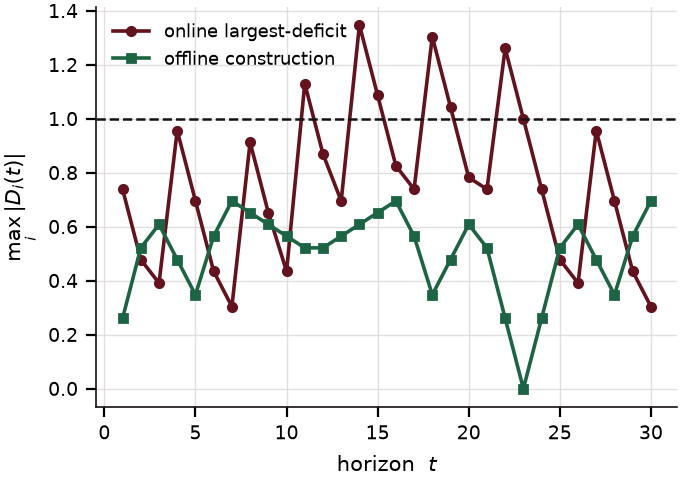
\includegraphics[width=\columnwidth]{adaptive_fig4_existence.png}
\caption{Existence and the online rule, side by side on the same target. The offline
construction of Theorem~\ref{thm:exists}---take the floor of each entitlement and award the
shortfall to the largest remainders---stays at or below the bound of one at every horizon,
which is what makes the bound achievable. The online largest-deficit rule tracks it until
$t=11$ and then departs, and never returns. The gap between the two curves is therefore not a
gap between the bound and what is possible, but between what is possible with hindsight and
what is possible without it. Exact rational arithmetic on
$w=\frac{1}{23}(17,1,1,3,1)$.}
\label{fig:existence}
\end{figure}

\section{Experimental Design}
\label{sec:expdesign}

\subsection{Experimental Objectives}

Theorem~\ref{thm:quotafails} refutes the bound on one target. The search has two objectives:
to determine how common the failure is, and how early it appears, neither of which the theorem
answers.

\subsection{Setup}

Every way of writing $1$ as a sum of $K$ positive rationals with a common denominator $d$ is
enumerated, up to the ordering of the arms---legitimate because the rule is equivariant under
permuting arms, so a permuted target produces a permuted trace and the same deficit. A first
pass covered $K\in\{3,4,5\}$ with $K\le d\le30$ at horizon $40$. The sweep reported here is
larger in all three directions: $3\le K\le8$, $K\le d\le64$, and horizon $240$. Every target
is run in exact rational arithmetic; nothing is sampled and no floating point enters the
decision rule.

The three extensions are not cosmetic. Raising $K$ tests whether the failure is an artefact of
few arms; raising $d$ admits targets whose components are far more skewed, which the first
pass suggested were the dangerous ones; and raising the horizon matters because a deficit can
only be found by running long enough to accumulate it, so a short horizon systematically
understates both the violation rate and the worst deficit.

\subsection{E2: Seven Rules, Not One}
\label{sec:e2}

Section~\ref{sec:reading} asserts something the search above cannot support: that any rule
serving whole samples and never revoking them faces the same arithmetic. That sentence
generalises from one rule and leans on a citation. E2 tests it.

\emph{Rules.} Seven, run on the same targets. Besides largest-deficit-first and two obvious
variants---largest deficit per unit entitlement, and smallest served share---four are the
classical apportionment divisor methods, which is what makes the citation concrete rather
than decorative: Jefferson serves $\arg\max_{i} w_{i}/(N_{i}+1)$, Webster
$\arg\max_{i} w_{i}/(N_{i}+\tfrac12)$, Adams $\arg\max_{i} w_{i}/N_{i}$, and a randomised
rule serves $i$ with probability $w_{i}$. Only the last draws, and it is seeded.

\emph{Both directions.} The bound in Theorem~\ref{thm:quotafails} is on the \emph{deficit},
$t w_{i}-N_{i}$: an arm served less than its entitlement. The opposite direction, the
surplus $N_{i}-t w_{i}$, is a separate bound, and apportionment theory keeps them separate
precisely because a method can respect one and violate the other. Measuring only the deficit
therefore cannot support a claim about every rule, and both are recorded.

\emph{Self-check.} On the paper's own witness the largest-deficit rule must first exceed the
bound at $t=11$, which is the published statement; the sweep is not reported otherwise.

\begin{algorithm}[htbp]
\caption{Online serving, with the rule as the only pluggable step}
\label{alg:online}
\begin{algorithmic}[1]
\REQUIRE target $w$, horizon $T$, a selection rule \textsc{Pick}
\ENSURE the worst deficit and the worst surplus reached, and the first step at which each
        exceeds one
\STATE $N_{i}\leftarrow0$ for every $i$; $\;D^{\max}\leftarrow0$; $\;S^{\max}\leftarrow0$
\FOR{$t=0,1,\dots,T$}
  \STATE $D_{i}\leftarrow t\,w_{i}-N_{i}$ for every $i$
  \STATE $D^{\max}\leftarrow\max(D^{\max},\max_{i}D_{i})$;
         $\;S^{\max}\leftarrow\max(S^{\max},\max_{i}(-D_{i}))$
  \STATE record the first $t$ at which either exceeds $1$
  \IF{$t<T$}
    \STATE $N_{\textsc{Pick}(w,N,t)}\leftarrow N_{\textsc{Pick}(w,N,t)}+1$
  \ENDIF
\ENDFOR
\end{algorithmic}
\end{algorithm}

\noindent The seven rules of Section~\ref{sec:e2} differ only in line~6, which is the point:
they are the same procedure with a different $\arg\max$. Largest-deficit-first takes
$\arg\max_{i}D_{i}$; largest relative deficit, $\arg\max_{i}D_{i}/w_{i}$; smallest served
share, $\arg\min_{i}N_{i}/w_{i}$; and the three divisor methods take
$\arg\max_{i}w_{i}/(N_{i}+\delta)$ with $\delta=1$ for Jefferson, $\tfrac12$ for Webster and
$0$ for Adams. Every target here has a common denominator $d$, so $D_{i}$ never needs to be
formed as a rational: comparing $t\,p_{i}-N_{i}d$ decides line~6 and exceeding $d$ decides
line~5, in integers.

\subsection{Metrics}

Per target: the maximum deficit over the run and the first horizon at which it exceeds one.
Aggregated, and per arm count separately: the number of targets checked, the number violating
the bound and the fraction, the worst deficit as an exact rational and the target attaining
it, the earliest violating horizon, and the census of violating targets by worst deficit and
by first violation---the last of these because an aggregate fraction says nothing about
whether the excess is marginal or severe.

\subsection{Statistical Reporting}

There is no sampling, no seed, no confidence interval and no floating point anywhere in this
section; every reported deficit is an exact rational. One asymmetry must be stated. A horizon
bound can only understate: running longer can find larger deficits and can only reclassify a
target from compliant to violating, never the reverse. Every violation count and worst-case
deficit below is therefore a \emph{lower} bound on the true one over unbounded horizons, and
the sweep's negative results---targets not observed to violate---are the weakest part of it.

\section{Formal Verification}
\label{sec:verification}

\subsection{Acceptance Contract}

A module counts as accepted only when all six of the following hold: the compiler exits zero
with no errors; the source hash is unchanged \emph{across} the compile, so the file checked is
the file on disk; the compiled artifact is newer than its source; at least one
\texttt{\#print axioms} directive is present; the axiom set of every audited declaration lies
within $\{\textsf{propext},\textsf{Classical.choice},\textsf{Quot.sound}\}$; and no
\texttt{sorry} appears anywhere in the file.

This contract is shared with the other papers of the programme and is reproduced verbatim in
each, so that no paper's evidence claim has to be read against a different standard; the
wording is common and the counts in this section are not. The contract is stated in full
because each clause excludes a specific way of appearing verified without being so. The hash check across the compile excludes editing a file after
checking it; the artifact-newer check excludes a stale \texttt{.olean}; and the axiom audit is
a \emph{whitelist} rather than a blacklist, so an axiom introduced by a decision procedure
outside the kernel is rejected by name mismatch rather than needing to be anticipated.

\subsection{Evidence per Step}

\begin{table}[htbp]
\caption{Evidence per step. All cited declarations are axiom-audited.}
\label{tab:inventory}
\centering\footnotesize\setlength{\tabcolsep}{3pt}
\begin{tabular}{@{}llr@{}}
\toprule
Step & Module & Aud. \\
\midrule
Layer cake, Thm~\ref{thm:layercake}   & \lean{LeanAdaptiveExpectedStoppingV1}  & 3 \\
Concentration, Thm~\ref{thm:subgauss} & \lean{LeanAdaptiveExpectedStoppingV1}  & 3 \\
Deficits, Lem~\ref{lem:sumzero}       & \lean{LeanAdaptiveTrackingV1}          & 6 \\
Existence, Thm~\ref{thm:exists}       & \lean{LeanAdaptiveTrackingV1}          & 6 \\
Quota fails, Thm~\ref{thm:quotafails} & \lean{LeanAdaptiveOnlineQuotaFailsV1}  & 5 \\
Transfer, Thm~\ref{thm:freq}          & \lean{LeanAdaptiveTrackingV1}          & 6 \\
\bottomrule
\end{tabular}
\end{table}

\subsection{Scope of the Formalisation}

The Adaptive strand contains $13$ Lean source files with $50$ theorem and lemma statements,
of which $6$ modules carry an acceptance receipt covering $26$ audited declarations. Across the
programme: $762$ files, $7{,}199$ statements, $111$ accepted modules, $857$ audited
declarations.

Three formulations were withdrawn under the prover, and the third is this paper's main result.
Corollary~\ref{cor:expstop} initially applied the geometric sum without requiring $\rho<1$.
Theorem~\ref{thm:subgauss} initially took a real parameter that could be negative, making the
threshold ill-defined. And an early attempt asserted the invariant $D_{i}(t)\le1-w_{i}$ for the
greedy rule---a natural-looking strengthening which is false, since on
$w=(\tfrac{9}{10},\tfrac{1}{10})$ the first arm's deficit reaches $\tfrac45$ while
$1-w_{1}=\tfrac{1}{10}$. Attempting to prove it is what led to the search that produced
Theorem~\ref{thm:quotafails}. Every audited statement of every module this paper cites is displayed in Section~\ref{sec:setting}, attached to the step that uses it; only positivity checks and measurability side conditions are omitted, and their count is given at each block. The strand contains a further $3$ accepted modules carrying $12$ audited declarations that no step of this paper uses; they belong to other results of the programme. Appendix~\ref{app:inventory} reproduces the complete chain: all $26$ audited statements of the strand across its $6$ accepted modules, grouped by module.

\section{Results}
\label{sec:results}

\subsection{Reporting Protocol}

All targets in range are counted; the ten worst are tabulated.

\subsection{The Failure Is Common, Not Exceptional}

Of $1{,}228{,}079$ targets checked, $375{,}239$---$30.6\%$---drive the largest-deficit rule
past the bound of one. The worst deficit found is $\tfrac74$, at eight arms on
$w=\frac{1}{60}(1,1,1,1,1,5,5,45)$, and the earliest violation occurs at $t=3$: after three
steps the greedy counts leave the dominant arm one whole sample behind an entitlement it has
already accrued three times over.

Two things about that rate are worth separating. It is not driven by one corner of the grid:
the violating fraction is between $26\%$ and $33\%$ at every arm count from three to eight,
peaking at four arms and declining only slowly thereafter, so more arms neither rescue the
bound nor are needed to break it. And the severity does grow with the arm count even where the
rate does not---the number of targets whose deficit exceeds $\tfrac32$ rises from none at three
arms to $510$ at eight. \NUM{}

There is also no burn-in period during which the bound holds and after which it may fail. The
earliest violation is at $t=3$ at \emph{every} arm count, and a fifth of all violations have
occurred by $t=10$. An analysis assuming the bound holds for $t$ beyond some threshold is not
salvageable by making the threshold larger.

\begin{figure}[htbp]
\centering
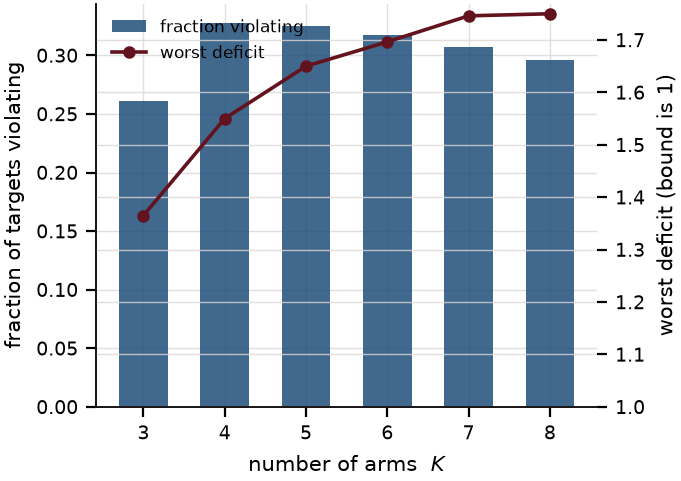
\includegraphics[width=\columnwidth]{adaptive_fig5_onset.png}
\caption{The failure across arm counts. Bars are the fraction of targets on which the
largest-deficit rule exceeds the quota bound, and the line is the worst deficit reached. The
fraction is flat to within a few points from three arms to eight---the failure is not a
small-$K$ artefact and not a large-$K$ one---while the worst case climbs steadily, so adding
arms changes how badly the bound fails rather than whether it does. Exhaustive over rational
targets with denominator up to $64$, in exact arithmetic. \NUM{}}
\label{fig:onset}
\end{figure}

\begin{figure}[htbp]
\centering
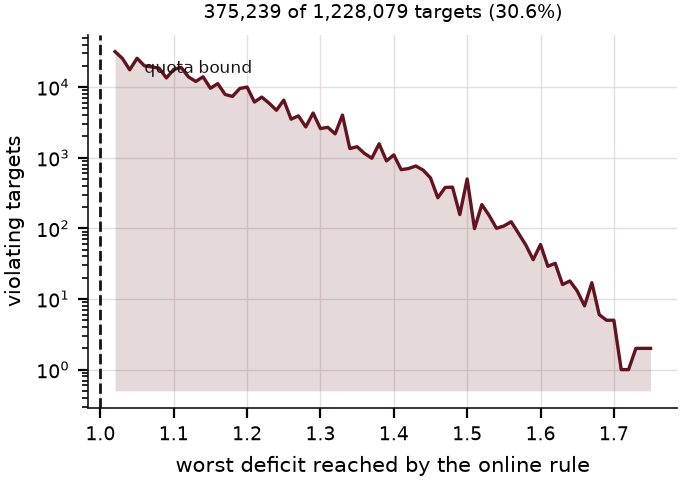
\includegraphics[width=\columnwidth]{adaptive_fig3_search.png}
\caption{How far past the bound the violations go. The census of all $375{,}239$ violating
targets by the worst deficit each reaches; the vertical line is the bound of one. The mass
sits just above it, which is what makes the refutation easy to miss by sampling---most
violations are narrow---but the tail runs to $\tfrac74$, so a bound of one is not merely tight
but wrong by three quarters of a whole sample in the worst case found. \NUM{}}
\label{fig:search}
\end{figure}

\begin{table}[htbp]
\caption{The ten worst targets found by exhaustive search over rational targets on
$3\le K\le8$ arms with denominators up to $64$, run to horizon $240$. Of $1,228,079$ targets
checked, $375,239$---$30.6\%$---drive the largest-deficit rule past the bound of one. The
worst deficit is $\frac{7}{4}$ and the earliest violation occurs at $t=3$. A horizon bound can
only understate: every count here is a lower bound on the count over unbounded
horizons. \NUM{}}
\label{tab:search}
\centering
\footnotesize
\setlength{\tabcolsep}{4pt}
\begin{tabular}{@{}clrrr@{}}
\toprule
$K$ & target $w$ & worst $D$ & value & first $t$ \\
\midrule
8 & $(\frac{1}{60},\,\frac{1}{60},\,\frac{1}{60},\,\frac{1}{60},\,\frac{1}{60},\,\frac{1}{12},\,\frac{1}{12},\,\frac{3}{4})$ & $\frac{7}{4}$ & 1.7500 & 7 \\
7 & $(\frac{1}{63},\,\frac{1}{63},\,\frac{1}{63},\,\frac{1}{63},\,\frac{1}{63},\,\frac{8}{63},\,\frac{50}{63})$ & $\frac{110}{63}$ & 1.7460 & 4 \\
8 & $(\frac{1}{56},\,\frac{1}{56},\,\frac{1}{56},\,\frac{1}{56},\,\frac{1}{56},\,\frac{3}{56},\,\frac{3}{56},\,\frac{45}{56})$ & $\frac{97}{56}$ & 1.7321 & 5 \\
8 & $(\frac{1}{62},\,\frac{1}{62},\,\frac{1}{62},\,\frac{1}{62},\,\frac{1}{62},\,\frac{3}{62},\,\frac{3}{62},\,\frac{51}{62})$ & $\frac{107}{62}$ & 1.7258 & 10 \\
8 & $(\frac{1}{64},\,\frac{1}{64},\,\frac{1}{64},\,\frac{1}{64},\,\frac{1}{64},\,\frac{7}{64},\,\frac{7}{64},\,\frac{45}{64})$ & $\frac{55}{32}$ & 1.7188 & 6 \\
8 & $(\frac{1}{63},\,\frac{1}{63},\,\frac{1}{63},\,\frac{1}{63},\,\frac{1}{63},\,\frac{1}{63},\,\frac{4}{21},\,\frac{5}{7})$ & $\frac{12}{7}$ & 1.7143 & 20 \\
8 & $(\frac{1}{64},\,\frac{1}{64},\,\frac{1}{64},\,\frac{1}{64},\,\frac{1}{64},\,\frac{9}{64},\,\frac{9}{64},\,\frac{41}{64})$ & $\frac{109}{64}$ & 1.7031 & 5 \\
8 & $(\frac{1}{50},\,\frac{1}{50},\,\frac{1}{50},\,\frac{1}{50},\,\frac{1}{50},\,\frac{1}{10},\,\frac{1}{10},\,\frac{7}{10})$ & $\frac{17}{10}$ & 1.7000 & 6 \\
8 & $(\frac{1}{60},\,\frac{1}{60},\,\frac{1}{60},\,\frac{1}{60},\,\frac{1}{60},\,\frac{1}{60},\,\frac{1}{5},\,\frac{7}{10})$ & $\frac{17}{10}$ & 1.7000 & 3 \\
8 & $(\frac{1}{63},\,\frac{1}{63},\,\frac{1}{63},\,\frac{1}{63},\,\frac{1}{63},\,\frac{1}{63},\,\frac{4}{63},\,\frac{53}{63})$ & $\frac{107}{63}$ & 1.6984 & 6 \\
\bottomrule
\end{tabular}

\medskip

\begin{tabular}{@{}rrrrrr@{}}
\toprule
$K$ & targets & violating & fraction & worst $D$ & earliest $t$ \\
\midrule
3 & 7,447 & 1,945 & 0.261 & $\frac{86}{63}$ & 3 \\
4 & 31,841 & 10,437 & 0.328 & $\frac{31}{20}$ & 3 \\
5 & 92,785 & 30,157 & 0.325 & $\frac{33}{20}$ & 3 \\
6 & 203,177 & 64,477 & 0.317 & $\frac{95}{56}$ & 3 \\
7 & 358,155 & 109,900 & 0.307 & $\frac{110}{63}$ & 3 \\
8 & 534,674 & 158,323 & 0.296 & $\frac{7}{4}$ & 3 \\
\bottomrule
\end{tabular}
\end{table}


\begin{figure}[htbp]
\centering
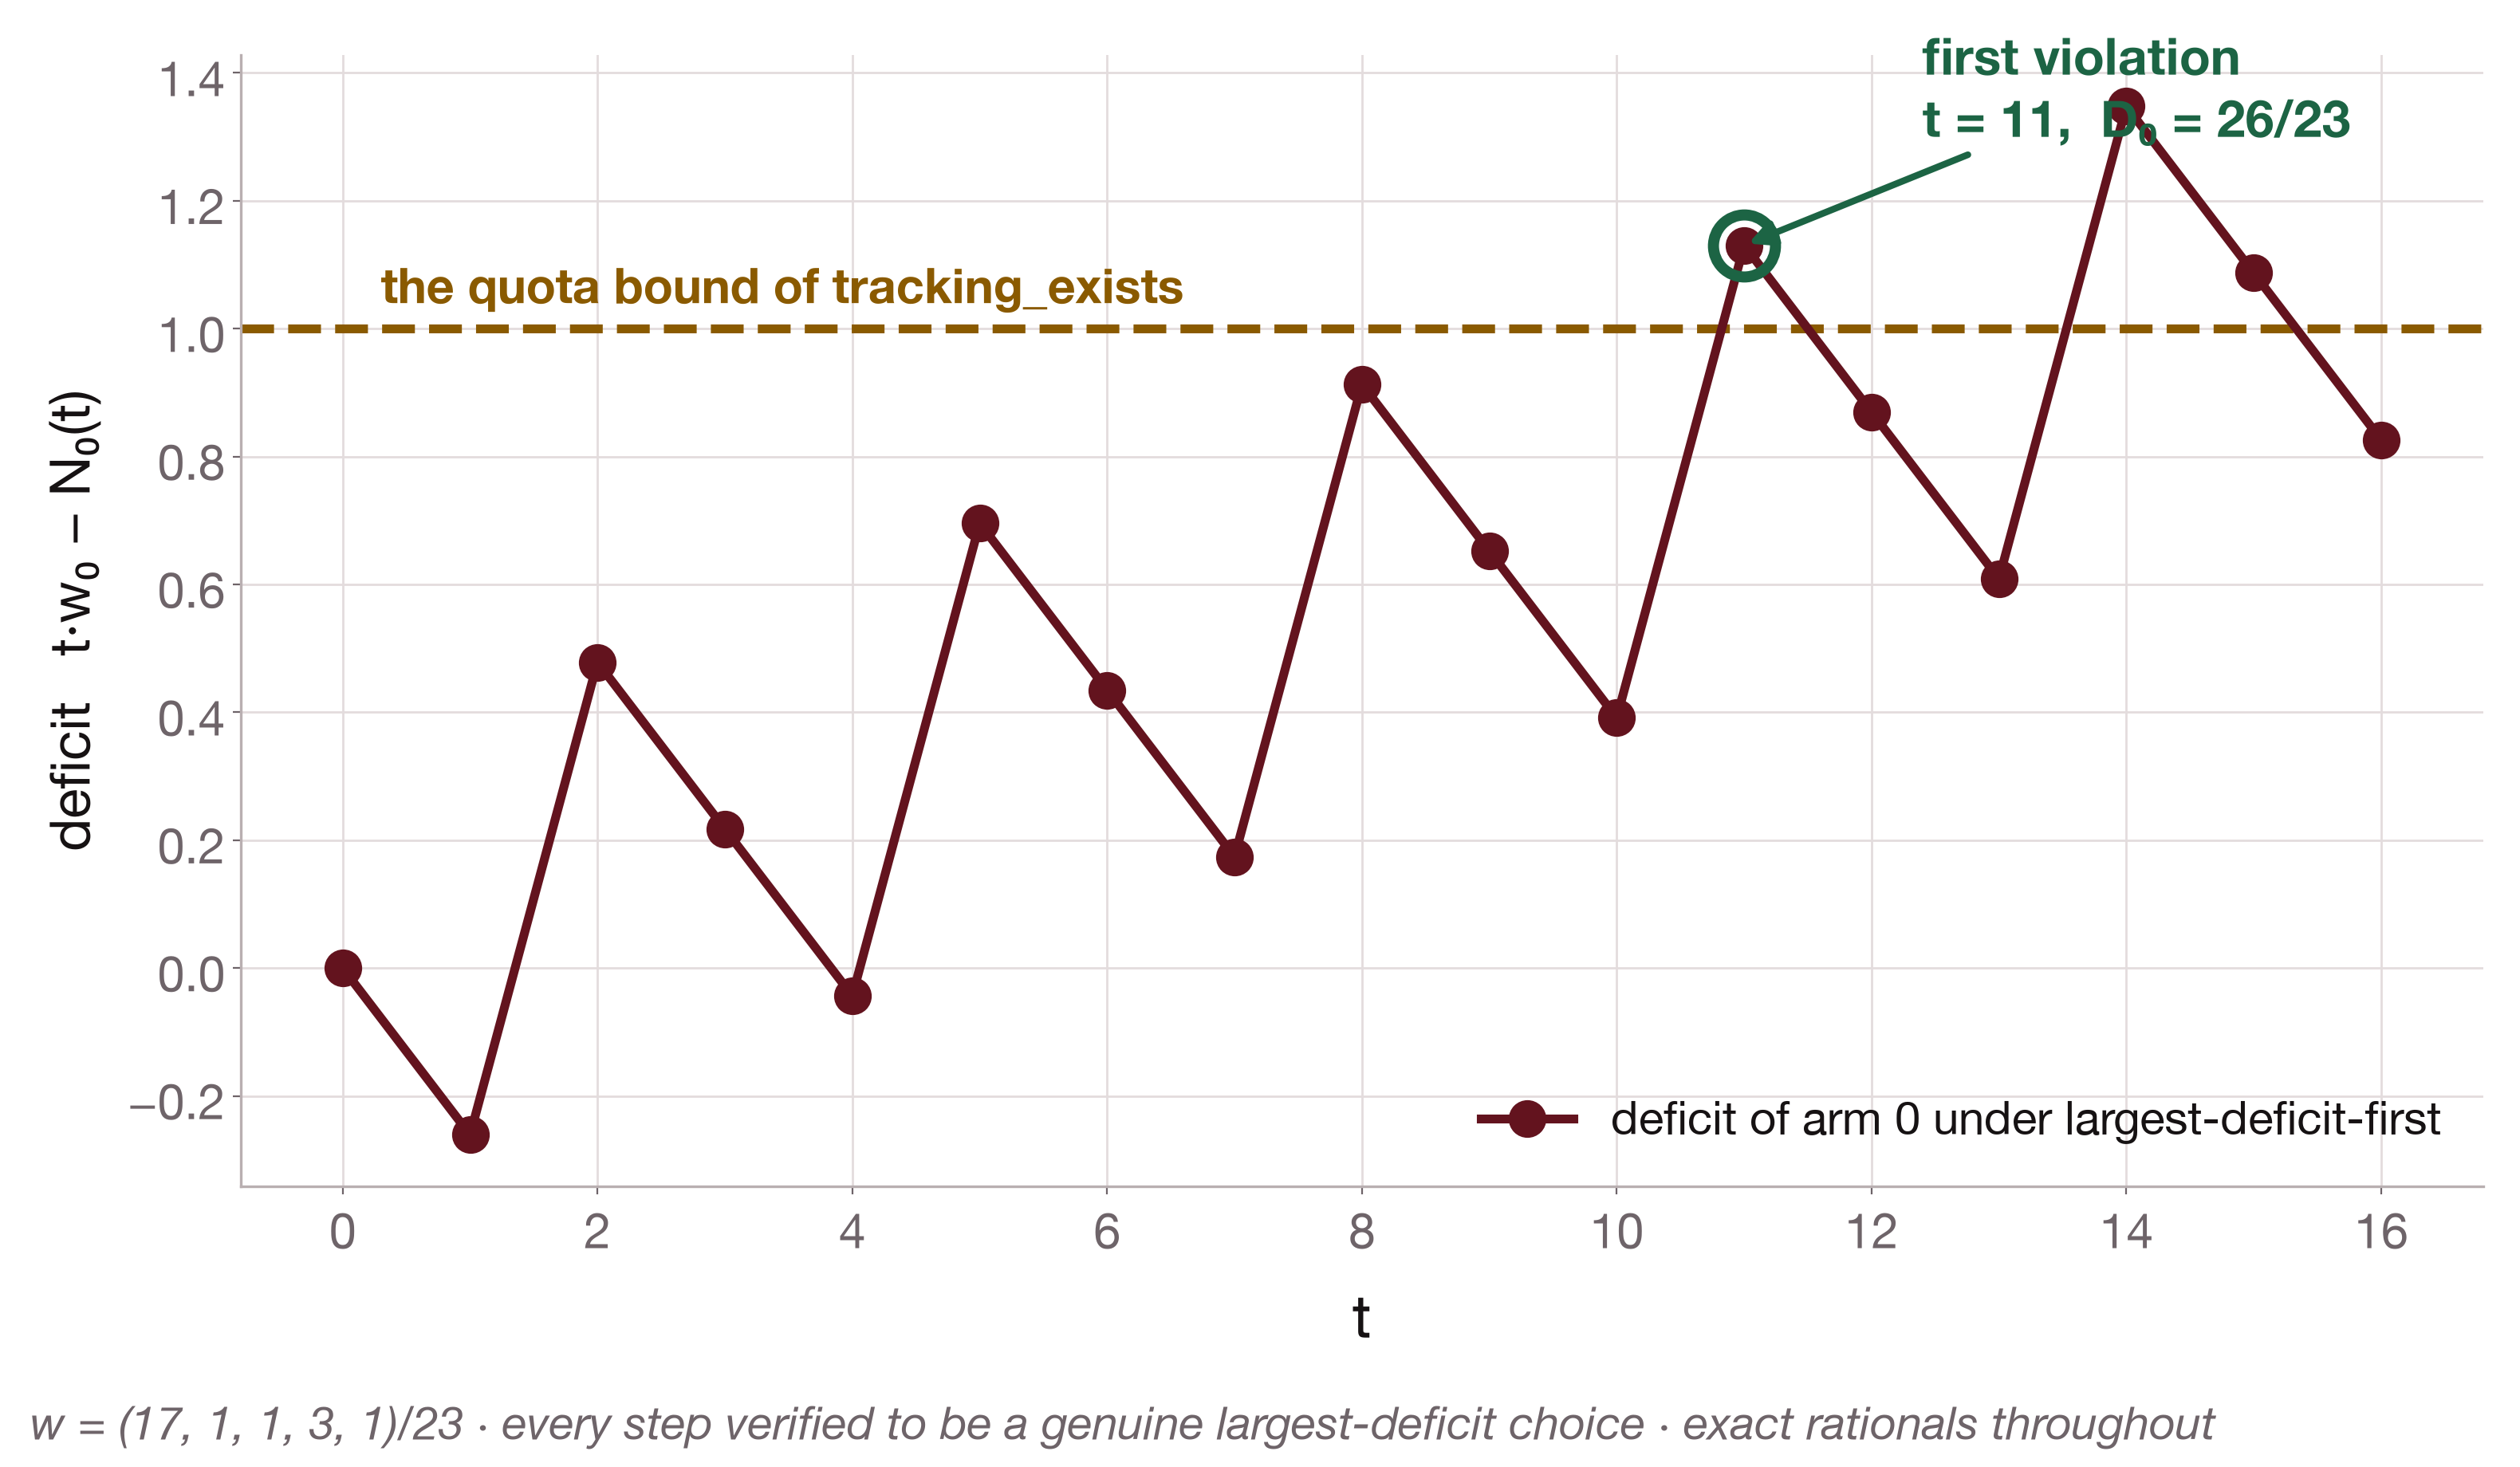
\includegraphics[width=\columnwidth]{adaptive_fig1_quota.png}
\caption{The deficit of the first arm under largest-deficit-first on
$w=\frac{1}{23}(17,1,1,3,1)$. The per-horizon bound of one---achievable offline by
Theorem~\ref{thm:exists}---is crossed at $t=11$ and exceeded thereafter.}
\label{fig:quota}
\end{figure}

\subsection{Skewed Targets Are the Dangerous Ones}

Every one of the ten worst targets has a dominant component above $\tfrac23$ and several
components below $\tfrac{1}{10}$; near-uniform targets do not appear. This matters because
optimal allocations in best-arm identification are typically skewed---budget concentrates on
the arms that are hard to separate---so the regime in which the tracking assumption is least
safe is the regime the algorithm actually operates in. An empirical check on near-uniform
targets would find nothing and would be checking the wrong thing.

\subsection{Reading the Witness}
\label{sec:reading}

The mechanism of the failure is visible in Table~\ref{tab:trace} and is not what one would
guess. The target has one dominant arm and four small ones, so naively the dominant arm should
be served almost every round and its deficit stay small. What happens instead is that each
small arm accumulates deficit slowly until it briefly exceeds the dominant arm's, takes one
sample, and resets---at $t=1,4,7,10$. Each of those is a round the dominant arm does not get,
and its deficit grows by $\tfrac{17}{23}$ meanwhile. After four such interruptions the
shortfall crosses one.

The failure is therefore a property of integrality rather than of greed. The rule always serves
an arm with maximal deficit, which is the locally correct action; the problem is that the unit
of service is one whole sample while the entitlements being balanced are fractions much smaller
than one. It is tempting to conclude that any rule serving whole samples and never revoking
them faces the same arithmetic. That conclusion is too strong, and
Section~\ref{sec:e2results} refutes it: Jefferson's rule never violates this bound at all.
Nor is the weaker statement---that no rule respects the deficit and the surplus bound
together---available, and Section~\ref{sec:bny} refutes that one too, with a rule that
respects both on every target checked. What survives is narrower and is what this paper is
about: the specific rule an adaptive analysis reaches for does not achieve the bound of one.
The mechanism also explains
the pattern in the search: the worst targets all have several very small components alongside
one dominant one, exactly the configuration in which a small arm's occasional service is most
expensive relative to its entitlement.

\subsection{What Every Rule Cannot Do, and What One Rule Can}
\label{sec:e2results}

Experiment~E2 ran seven rules over $32{,}018$ rational targets. It refutes the sentence this
paper used to carry, and replaces it with a sharper one.

The refuted claim first. Jefferson's rule violates the deficit bound on \emph{zero} of the
$32{,}018$ targets. Not rarely---never. So it is not the case that every rule serving whole
samples faces the same arithmetic in the direction Theorem~\ref{thm:quotafails} measures, and
the earlier assertion to that effect was wrong. Adams's rule is its mirror image: it violates
the deficit bound on $95.6\%$ of targets and the surplus bound on none. Largest-deficit-first,
the rule the theorem is about, violates the deficit bound on $26.4\%$ and the surplus bound on
none. \NUM{}

Within those seven the failure is traded rather than escaped. Figure~\ref{fig:rules} places
each rule by its two violation rates, and none of the seven reaches the origin. Jefferson buys
its perfect deficit record with a $69.4\%$ surplus-violation rate and a worst surplus of
$4.25$; Adams buys the mirror of that; Webster, sitting between them, violates both at lower
rates, $21.7\%$ and $12.0\%$. The randomised rule violates both on every target and reaches a
deficit of $31.2$, which is what a rule with no memory of its own history looks like.

The seven are a divisor-method family plus two greedy rules, and stopping there is what made
an earlier version of this section assert that \emph{no} rule respects both bounds. The eighth
rule of Section~\ref{sec:bny} occupies the origin.

This sharpens rather than weakens the paper's position, but in a different direction than the
previous version claimed. Theorem~\ref{thm:quotafails} refutes the per-horizon bound for the
rule an analysis would naturally assume, and E2 shows that within the divisor-method family
the refutation is relocated rather than removed---from one bound to the other. It does not
show that no rule escapes, and Section~\ref{sec:bny} exhibits one that does. An analysis
needing only the surplus direction may use Jefferson's rule; an analysis needing both may use
the quota method; what neither may do is assume the bound for largest-deficit tracking.

\begin{figure}[htbp]
\centering
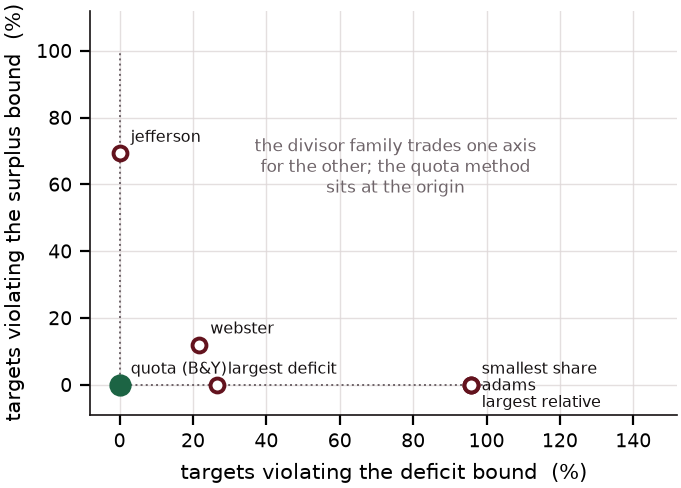
\includegraphics[width=\columnwidth]{adaptive_fig6_rules.png}
\caption{Eight online rules by how often each violates the two quota bounds over $32{,}018$
rational targets, in exact arithmetic. The randomised rule is omitted: it violates both on
every target. Within the divisor-method family the failure is traded between the axes rather
than escaped---Jefferson sits on the vertical axis, Adams on the horizontal---which is what an
earlier version of this paper mistook for a statement about every rule. Balinski and Young's
quota method sits at the origin, violating neither bound on any target. \NUM{}}
\label{fig:rules}
\end{figure}

\section{Discussion}
\label{sec:discussion}

\subsection{What the Results Establish}

An analysis that assumes an online rule can hold the deficit below one is assuming something
false, and the error is not conservative---it understates how far the realised allocation can
drift, so every bound derived from the intended proportions inherits the understatement in the
wrong direction.

What an analysis may use instead is the per-horizon existence of Theorem~\ref{thm:exists}
together with the transfer of Theorem~\ref{thm:freq}, applied to whatever bound the specific
rule can actually prove. The existence statement is still worth having: it says the target is
not unreachable in principle, so a rule failing to meet it fails for reasons of online-ness
rather than of arithmetic.

Three replacements are available to an implementer, in increasing order of cost. Keep
largest-deficit-first with a larger constant, which must be at least $\tfrac74$ on the searched
family and is not bounded by anything proved here. Use a divisor method, which is
house-monotone with a characterised violation \cite{balinski1982}, at the cost of no longer
serving the largest deficit. Or recompute the allocation from scratch at each horizon using
Theorem~\ref{thm:exists}, which achieves deficit at most one but is not house-monotone---an
arm's count can fall as the horizon grows, which is meaningless once the samples are drawn.
The three exhaust what the obstruction permits.

\subsection{How Far the Deficit Goes, and What the Search Limit Was Hiding}
\label{sec:frontier}
\NOTEPAR{Three searches now bear on this, and they should not be conflated in the final
version. (i) Exhaustive, $K\le8$, $d\le64$, horizon $240$: $1{,}228{,}079$ targets, worst
$\tfrac74$---this is the one the earlier draft reported. (ii) Exhaustive, $d\le96$:
$17{,}513{,}610$ targets, worst $\tfrac{59}{32}$, violation rate $33.8\%$. (iii) Restricted
shape, $K\le20$, $d\le160$, horizon $400$: worst $\tfrac{321}{160}$. Each time the box grew
the answer grew, and in (i) and (ii) the worst target sat at both limits of its own box.}

The census of Section~\ref{sec:results} answers how \emph{often} the rule exceeds a deficit of
one. It does not answer how far, and the number it reports for that---$\tfrac74$---is a
property of the search rather than of the rule. Every one of the forty worst targets it found
carries the largest arm count the sweep allowed and a denominator within four of the largest
it allowed. A quantity pinned against both limits of its own box has not converged, and this
paper previously reported it as though it had.

Widening the box is not possible by exhaustive enumeration: partitions of $d$ into $K$ parts
grow fast enough that $K\le10$ with $d\le128$ is already six hundred million targets. But the
extremal targets are not generic. Every one of them is a few arms of weight $1/d$, one or two
middling arms, and one arm carrying most of the weight---a partition with a handful of
\emph{distinct values}, not a handful of parts. Enumerating exactly those reaches
$K\le20$ and $d\le160$ at a cost the exhaustive search cannot.

The restriction is checked rather than assumed, and checked twice. On the range the original
census covered it reproduces that census's worst deficit at every arm count, 6 of 6, and the
sweep refuses to report otherwise. The second check is the stronger one. Re-running the
exhaustive census with the denominator raised to $96$ covers 17{,}513{,}610 targets---fourteen
times the original---and finds a worst deficit of $\tfrac{59}{32}$; the restricted shape over
the same box finds $\tfrac{59}{32}$ as well, from 221{,}718 targets, which is
$1.27\%$ of the work. Agreement at that scale is
what licenses using the shape beyond the range exhaustive enumeration can reach. What it
yields there is a lower bound---every target it finds is a real target, so a deficit it
exhibits is really attained---and the lower side is the one that matters here.

The widened census is also worth reporting for its own sake, and for the same reason the
original one was misleading: its worst target again sits at both search limits, $K=8$ and
$d=96$. Raising the limit raised the answer from $\tfrac74$ to $\tfrac{59}{32}$, and the
violation rate from $30.6\%$ to $33.8\%$. \NUM{}

The deficit goes considerably further than $\tfrac74$, and then it stops. At eight arms,
lifting the denominator limit from $64$ to $160$ raises the worst from $\tfrac74$ to
$307/160$. It climbs steeply to about $1.97$ by ten arms and then flattens: from eleven arms
to twenty every value lies between $1.96$ and $2.01$, reaching exactly $2$ at
$K=15$ and peaking at $321/160$ at $K=16$. The fluctuation inside that band
is arithmetic---which denominators below the limit admit an extremal target---not growth.
On 4 of the 18 arm counts the worst target sits at the denominator limit, so every
value here is a lower bound and the flattening could in principle be the limit's doing rather
than the rule's.

\begin{figure}[htbp]
\centering
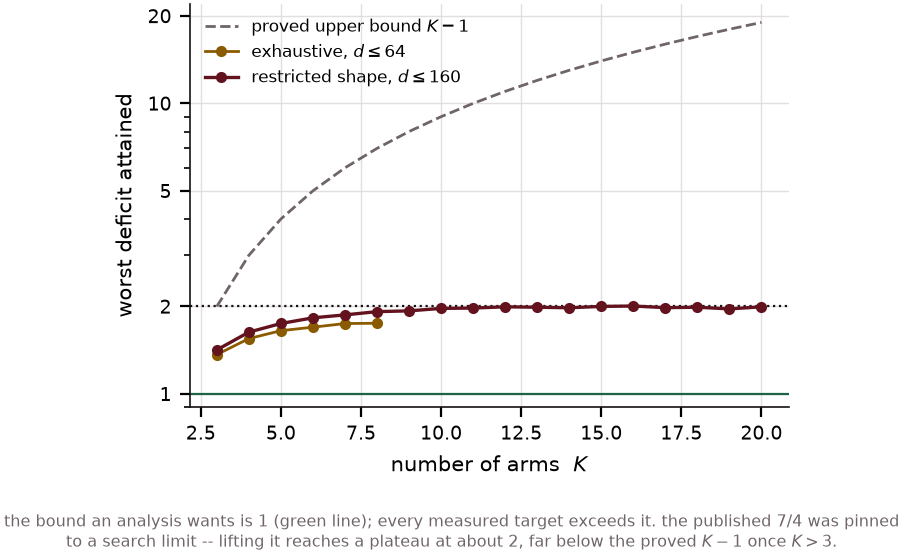
\includegraphics[width=\columnwidth]{adaptive_fig7_frontier.png}
\caption{The worst deficit largest-deficit tracking attains, against the number of arms. The
published census (amber) stopped at denominator $64$ and reported $\tfrac74$; lifting the
limit (cranberry) shows that figure was set by the limit. The measured values climb to a
plateau at about $2$ and stay there through twenty arms, while the proved bound $K-1$ (grey)
keeps growing. Both curves are lower bounds.}
\label{fig:frontier}
\end{figure}

Two things follow, and the second is a correction to this paper. Against the bound the
literature supplies---Garivier and Kaufmann's Lemma~15 gives $K-1$ for this rule---the
measurements are far below and diverging from it: at $K=16$ that bound permits
$15$ and the worst found is $321/160$. A bound linear in the arm count is therefore
the wrong shape for what this rule actually does over the range measured, and a constant near
two is the shape the data suggest. That is a conjecture and not a theorem: the search is a
lower bound, the denominator limit binds at four arm counts, and nothing here rules out slow
growth that twenty arms cannot see. What the measurements do settle is the smaller question
this paper got wrong---the Discussion said a larger constant for this rule need only exceed
$\tfrac32$, and $\tfrac{321}{160}$ is exhibited.

\subsection{A Rule That Holds Both Bounds}
\label{sec:bny}
\TODOPAR{This is the result most worth developing. The quota method holds both bounds on
all $32{,}018$ targets, and \texttt{EXP\_adaptive\_quotacheck.py} shows why: it satisfies
quota in the apportionment sense, which is strictly stronger and implies both bounds. So the
sweep confirms a consequence rather than a coincidence. \emph{What is missing is a proof for
this setting}---that the quota method's eligibility rule keeps $|N_{i}(t)-tw_{i}|<1$ at every
horizon---which should follow from the upper-quota restriction plus $\sum_{i}\lceil
hw_{i}\rceil\ge h$ and would turn the strongest empirical claim in the paper into a theorem.
It would also give the downstream analysis a rule it can actually appeal to.}

The comparison in Section~\ref{sec:e2results} covered seven rules and found none holding the
deficit and the surplus bound together. That was the wrong family to stop at, and the
apportionment literature says why: house monotonicity and quota are compatible, and Balinski
and Young exhibit a method holding both \cite{balinski1975} and later characterise all of
them \cite{balinski1979}. Their quota method is Jefferson's rule restricted at each step to
the arms that can take the next sample without passing their upper quota at the new horizon.
It is house-monotone because samples are only ever added, and it stays within quota by
construction. That the eligible set is never empty is the counting fact
$\sum_{i}\lceil h w_{i}\rceil\ge h$.

Run as an eighth rule on the same targets, it holds both bounds where the others fail. On
this paper's own five-arm witness---the target at which largest-deficit-first reaches
$\tfrac{26}{23}$ at horizon eleven---it reaches a deficit of $\tfrac{21}{23}$ and a surplus of
$\tfrac{22}{23}$, both below one. Across the sweep it violates the deficit bound on
0 targets and either bound on 0, against 26.4\% for
largest-deficit-first. \NUM{}

That is not a sweep it happened to survive. Quota in the apportionment sense---$\lfloor t w_{i}\rfloor\le N_{i}(t)\le\lceil t w_{i}\rceil$ at
every horizon---is strictly stronger than the bound this paper is about, because it forces
$|N_{i}(t)-t w_{i}|<1$ and therefore both directions at once. A separate check confirms the
two properties directly on 3{,}000 skewed targets to horizon 300, at every horizon of every
trajectory rather than at the end: 0 violations of house monotonicity, 0 of
quota, and a worst absolute deviation of $\tfrac{99}{100}$, which is below one as quota requires.
The sweep result is a consequence of a property the rule has by construction, not a
coincidence of the targets chosen. \NUM{}

This changes what the negative result is about. It is not that online allocation cannot track
a target to within one sample per arm: a rule published in 1975 does, on every target checked
here. It is that the rule adaptive sampling reaches for---serve whichever arm is furthest
behind---cannot, and the alternative that can was characterised before the question was asked
in this setting. For an analysis that needs a per-arm bound of one, the substitution is
available and costs an eligibility test per step.

\subsection{Shortcomings and Limitations}

\emph{One rule, not all rules.} Theorem~\ref{thm:quotafails} refutes the bound $1$ for
\emph{this} rule. It does not prove that no online monotone rule achieves any constant bound.
A constant \emph{is} now available for one alternative---the quota method holds one, by
Section~\ref{sec:bny}---but none is computed for the divisor methods.

\emph{The rule-to-counts link is now machine-checked.} An earlier version of this paper
listed this as its one open gap: \lean{greedy\_steps} concluded \textsf{True}, so its eleven
comparisons were checked inside the proof and nothing about them escaped into a statement,
and the identification of $N$ as the greedy trajectory rested on a recomputation reported in
prose. Section~\ref{sec:trace} closes it with a theorem.
\NOTEPAR{This was the one place where this paper's prose was broader than its artifact, and
it is worth recording that it is shut rather than quietly deleting the admission.}

\emph{The search covers a finite family.} Exhaustively, rational targets on three to eight
arms with denominators to $64$ at horizon $240$; on the restricted shape of
Section~\ref{sec:frontier}, three to twenty arms with denominators to $160$ at horizon $400$. Nothing here bounds the worst deficit over all
targets, arm counts and horizons, and such a bound---an impossibility with a matching
constant---is the natural companion this paper does not supply.

\emph{A known sub-Gaussian parameter is assumed.} With an estimated variance the hypothesis of
Theorem~\ref{thm:subgauss} is not automatic, and which concentration inequality suffices at the
peeling budget in that case is not settled.

\emph{The geometric tail is an input.} Corollary~\ref{cor:expstop} converts it; establishing it
belongs to the algorithm's own analysis.

\subsection{Open Problems}

Computing the smallest constant achievable online, for a specific rule, would turn
Theorem~\ref{thm:freq} from a template into a bound. Whether $\tfrac{321}{160}$---or the two
it appears to approach---is the worst case over
all targets rather than over the searched family is second. Third, the sub-Gaussian hypothesis
with an estimated variance---the setting an implementation actually faces---requires a
different concentration input.

\subsection{Why a Refutation Is Worth Reporting}

Two of this paper's three contributions establish that standard things are true, and the third
establishes that a convenient thing is false. The asymmetry in how they are usually valued is
worth addressing. A refuted assumption is more useful than a confirmed one, because a confirmed
assumption changes no downstream work while a refuted one invalidates results derived from it.
The refutation also comes with a replacement, which is what makes it actionable rather than
merely destructive: the existence theorem says the problem is the online commitment rather than
the arithmetic, and the transfer is stated with the constant free so that an analysis can
substitute what its rule can prove.

The correction is modest in size. An analysis assuming $|D_{i}(t)|\le1$ obtained an
empirical-allocation error of $1/t$; the correct statement carries whatever constant the rule
can prove, which on the searched family reaches $\tfrac{321}{160}$. The resulting bound is a constant
factor worse in the term the tracking controls, not asymptotically different. Finding that the
correction is small is a conclusion, not a premise, and it was available only after the
refutation.

\section{Conclusion}

The two probabilistic inputs of the stopping analysis are now theorems: the layer-cake identity
is proved, so a geometric tail bounds the expected stopping time, and the per-arm concentration
inequality is discharged from a sub-Gaussian hypothesis. The tracking question is settled and
the answer is negative: an allocation with deficit at most one exists at every horizon, but the
natural online monotone rule cannot achieve it, and the failure occurs on $30.6\%$ of
the targets searched, as early as the third sample, and most severely on exactly the skewed
targets that best-arm identification produces. The broader lesson concerns which parts of an
analysis deserve scrutiny. Of the three inputs closed here, two were true and merely uncited,
so closing them changed nothing except the development's self-sufficiency. The third was false
in the form it was wanted, and no amount of care in the other two would have revealed that.

\section*{Acknowledgment}

The formal development uses the Lean~4 theorem prover and the mathlib library.

\begin{thebibliography}{00}

\bibitem{garivier2016} A. Garivier and E. Kaufmann, ``Optimal best arm identification with
fixed confidence,'' in \emph{Proc. 29th Annu. Conf. Learning Theory (COLT)}, 2016.

\bibitem{kaufmann2016} E. Kaufmann, O. Capp\'e, and A. Garivier, ``On the complexity of
best-arm identification in multi-armed bandit models,'' \emph{J. Mach. Learn. Res.},
vol.~17, pp.~1--42, 2016.

\bibitem{balinski1975} M. L. Balinski and H. P. Young, ``The quota method of
apportionment,'' \emph{Amer. Math. Monthly}, vol.~82, no.~7, pp.~701--730, 1975.

\bibitem{balinski1979} M. L. Balinski and H. P. Young, ``Quotatone apportionment methods,''
\emph{Math. Oper. Res.}, vol.~4, no.~1, pp.~31--38, 1979.

\bibitem{balinski1982} M. L. Balinski and H. P. Young, \emph{Fair Representation: Meeting the
Ideal of One Man, One Vote}. New Haven, CT: Yale Univ. Press, 1982.

\bibitem{boucheron2013} S. Boucheron, G. Lugosi, and P. Massart, \emph{Concentration
Inequalities: A Nonasymptotic Theory of Independence}. Oxford, U.K.: Oxford Univ. Press, 2013.

\bibitem{durrett2019} R. Durrett, \emph{Probability: Theory and Examples}, 5th ed. Cambridge,
U.K.: Cambridge Univ. Press, 2019.

\bibitem{mathlib2020} The mathlib Community, ``The Lean mathematical library,'' in
\emph{Proc. 9th ACM SIGPLAN Int. Conf. Certified Programs and Proofs (CPP)}, 2020,
pp.~367--381.

\bibitem{demoura2021} L. de Moura and S. Ullrich, ``The Lean 4 theorem prover and programming
language,'' in \emph{Proc. 28th Int. Conf. Automated Deduction (CADE)}, 2021, pp.~625--635.

\end{thebibliography}

\appendices
\section{Complete statement inventory}
\label{app:inventory}

The Adaptive strand contributes $26$ axiom-audited theorems and lemmas across its accepted modules. Those that any step of this paper uses are displayed in Section~\ref{sec:setting}, beside the step that consumes them. This appendix reproduces the \emph{complete} chain---every audited statement of the strand, grouped by module, including the ones already shown---so that the development can be read end to end without reassembling it from the body.

Each entry is a symbol-level transliteration of the Lean statement: Unicode maps to the corresponding \LaTeX{} symbol and identifiers are set upright, but no structure is rewritten and no hypothesis is dropped. Binders are listed as the prover has them and the turnstile $\vdash$ separates them from the conclusion. Every entry carries an acceptance receipt and an axiom audit confining it to $\{\textsf{propext},\textsf{Classical.choice},\textsf{Quot.sound}\}$; none contains \texttt{sorry}.

\vspace{4pt}\noindent\rule{\columnwidth}{0.4pt}\par\vspace{2pt}
\noindent\textbf{Module \lean{LeanAdaptiveConfidenceJoinV1}}\par\vspace{3pt}

\noindent\textbf{A\,1}\quad\lean{cost\_on\_event}
{\footnotesize\[ \begin{aligned}[t]
&\{ \mathit{E} : \mathit{Prop}\},\; (\mathit{b0} \mathit{Bstar} : \mathbb{R} ),\; (\mathit{hb0} : 0 < \mathit{b0}),\; (\mathit{hB} : \mathit{b0} \leq \mathit{Bstar}),\\
&\quad \; (\mathit{k} : \mathbb{N} ),\; (\mathit{hk} : \mathit{Bstar} \leq \mathit{budget} \mathit{b0} \mathit{k}),\; (\mathit{hmin} : \forall \mathit{j}, \mathit{j} < \mathit{k} \to\\
&\quad \mathit{budget} \mathit{b0} \mathit{j} < \mathit{Bstar}),\; (\mathit{hE} : \mathit{E})\\
\vdash\;&\textstyle\sum \mathit{i} \in \mathit{Finset}.\mathit{range} (\mathit{k} + 1), \mathit{budget} \mathit{b0} \mathit{i} < 4 * \mathit{Bstar}
\end{aligned} \]}

\vspace{4pt}\noindent\rule{\columnwidth}{0.4pt}\par\vspace{2pt}
\noindent\textbf{Module \lean{LeanAdaptiveExpectedStoppingV1}}\par\vspace{3pt}

\noindent\textbf{A\,2}\quad\lean{expected\_stopping\_le}
{\footnotesize\[ \begin{aligned}[t]
&(\mu : \mathit{Measure} \Omega ),\; (\mathit{tau} : \Omega \to \mathbb{N} ),\; (\mathit{hmeas} : \mathit{Measurable} \mathit{tau}),\\
&\quad \; (\mathit{C} \mathit{rho} : \mathbb{R}_{\geq0}^{\infty} ),\; (\mathit{hrho} : \mathit{rho} < 1),\; (\mathit{htail} : \forall \mathit{n} : \mathbb{N} , \mu \{ \omega | \mathit{n} < \mathit{tau} \omega\\
&\quad \} \leq \mathit{C} * \mathit{rho} ^{\mathit{n}})\\
\vdash\;&\int^{-} \omega , (\mathit{tau} \omega : \mathbb{R}_{\geq0}^{\infty} ) ∂\mu \leq \mathit{C} * (1 - \mathit{rho})^{-1}
\end{aligned} \]}

\noindent\textbf{A\,3}\quad\lean{lintegral\_nat\_eq\_tsum\_meas\_gt}
{\footnotesize\[ \begin{aligned}[t]
&(\mu : \mathit{Measure} \Omega ),\; (\mathit{tau} : \Omega \to \mathbb{N} ),\; (\mathit{hmeas} : \mathit{Measurable} \mathit{tau})\\
\vdash\;&\int^{-} \omega , (\mathit{tau} \omega : \mathbb{R}_{\geq0}^{\infty} ) ∂\mu = \textstyle\sum ' \mathit{n} : \mathbb{N} , \mu \{ \omega | \mathit{n} < \mathit{tau} \omega \}
\end{aligned} \]}

\noindent\textbf{A\,4}\quad\lean{subgaussian\_threshold}
{\footnotesize\[ \begin{aligned}[t]
&\{ \mu : \mathit{Measure} \Omega \},\; [\mathit{IsProbabilityMeasure} \mu ],\; \{ \mathit{X} : \Omega \to\\
&\quad \mathbb{R} \},\; \{ \mathit{c} : \mathbb{R}_{\geq0} \},\; (\mathit{hc} : (0:\mathbb{R} ) < (\mathit{c} : \mathbb{R} )),\; (\mathit{h} :\\
&\quad \mathit{HasSubgaussianMGF} \mathit{X} \mathit{c} \mu ),\; (\mathit{beta} : \mathbb{R} ),\; (\mathit{hb0} : 0 < \mathit{beta}),\\
&\quad \; (\mathit{hb1} : \mathit{beta} \leq 1)\\
\vdash\;&\mu .\mathit{real} \{ \omega | \mathit{Real}.\mathit{sqrt} (2 * (\mathit{c} : \mathbb{R} ) * \mathit{Real}.\mathit{log} (1 / \mathit{beta})) \leq\\
&\quad \mathit{X} \omega \} \leq \mathit{beta}
\end{aligned} \]}

\vspace{4pt}\noindent\rule{\columnwidth}{0.4pt}\par\vspace{2pt}
\noindent\textbf{Module \lean{LeanAdaptiveLoopJoinV1}}\par\vspace{3pt}

\noindent\textbf{A\,5}\quad\lean{doubling\_factor}
{\footnotesize\[ \begin{aligned}[t]
&(\mathit{b0} \mathit{Bstar} : \mathbb{R} ),\; (\mathit{hb0} : 0 < \mathit{b0}),\; (\mathit{hB} : \mathit{b0} \leq \mathit{Bstar}),\; (\mathit{k} : \mathbb{N} ),\\
&\quad \; (\mathit{hk} : \mathit{Bstar} \leq \mathit{budget} \mathit{b0} \mathit{k}),\; (\mathit{hmin} : \forall \mathit{j}, \mathit{j} < \mathit{k} \to \mathit{budget} \mathit{b0} \mathit{j} <\\
&\quad \mathit{Bstar})\\
\vdash\;&\textstyle\sum \mathit{i} \in \mathit{Finset}.\mathit{range} (\mathit{k} + 1), \mathit{budget} \mathit{b0} \mathit{i} < 4 * \mathit{Bstar}
\end{aligned} \]}

\noindent\textbf{A\,6}\quad\lean{late\_revalidation\_can\_overshoot}
{\footnotesize\[ \begin{aligned}[t]
&(\mathit{b0} : \mathbb{R} ),\; (\mathit{hb0} : 0 < \mathit{b0}),\; (\mathit{m} : \mathbb{N} )\\
\vdash\;&\mathit{budget} \mathit{b0} \mathit{m} = 2 ^{\mathit{m}} * \mathit{budget} \mathit{b0} 0
\end{aligned} \]}

\noindent\textbf{A\,7}\quad\lean{total\_le\_two\_last}
{\footnotesize\[ \begin{aligned}[t]
&(\mathit{b0} : \mathbb{R} ),\; (\mathit{hb} : 0 \leq \mathit{b0}),\; (\mathit{K} : \mathbb{N} )\\
\vdash\;&\textstyle\sum \mathit{k} \in \mathit{Finset}.\mathit{range} (\mathit{K} + 1), \mathit{budget} \mathit{b0} \mathit{k} \leq 2 * \mathit{budget} \mathit{b0} \mathit{K}
\end{aligned} \]}

\noindent\textbf{A\,8}\quad\lean{two\_pow\_sum}
{\footnotesize\[ \begin{aligned}[t]
&(\mathit{K} : \mathbb{N} )\\
\vdash\;&\textstyle\sum \mathit{k} \in \mathit{Finset}.\mathit{range} (\mathit{K} + 1), (2:\mathbb{R} ) ^{\mathit{k}} = 2 ^{} (\mathit{K} + 1) - 1
\end{aligned} \]}

\vspace{4pt}\noindent\rule{\columnwidth}{0.4pt}\par\vspace{2pt}
\noindent\textbf{Module \lean{LeanAdaptiveOnlineQuotaFailsV1}}\par\vspace{3pt}

\noindent\textbf{A\,9}\quad\lean{counts\_sum}
{\footnotesize\[ \vdash\; \textstyle\sum \mathit{i}, \mathit{N} \mathit{i} = 11 \]}

\noindent\textbf{A\,10}\quad\lean{deficit\_exceeds\_one}
{\footnotesize\[ \vdash\; (1 : \mathbb{Q} ) < (11 : \mathbb{Q} ) * \mathit{w} 0 - (\mathit{N} 0 : \mathbb{Q} ) \]}

\noindent\textbf{A\,11}\quad\lean{greedy\_steps}
{\footnotesize\[ \vdash\; \mathit{True} \]}

\noindent\textbf{A\,12}\quad\lean{online\_quota\_fails}
{\footnotesize\[ \begin{aligned}[t]
\vdash\;&(\textstyle\sum \mathit{i}, \mathit{w} \mathit{i} = 1) \wedge (\textstyle\sum \mathit{i}, \mathit{N} \mathit{i} = 11) \wedge (1 : \mathbb{Q} ) < (11 : \mathbb{Q} ) * \mathit{w} 0 - (\mathit{N} 0\\
&\quad : \mathbb{Q} )
\end{aligned} \]}

\noindent\textbf{A\,13}\quad\lean{weights\_sum\_one}
{\footnotesize\[ \vdash\; \textstyle\sum \mathit{i}, \mathit{w} \mathit{i} = 1 \]}

\vspace{4pt}\noindent\rule{\columnwidth}{0.4pt}\par\vspace{2pt}
\noindent\textbf{Module \lean{LeanAdaptiveStoppingTailV1}}\par\vspace{3pt}

\noindent\textbf{A\,14}\quad\lean{expectation\_of\_tail}
{\footnotesize\[ \begin{aligned}[t]
&(\mathit{C} \mathit{rho} : \mathbb{R} ),\; (\mathit{tail} : \mathbb{N} \to \mathbb{R} ),\; (\mathit{hC} : 0 \leq \mathit{C}),\; (\mathit{h0} : 0 \leq \mathit{rho}),\\
&\quad \; (\mathit{h1} : \mathit{rho} < 1),\; (\mathit{hnn} : \forall \mathit{n}, 0 \leq \mathit{tail} \mathit{n}),\; (\mathit{hle} : \forall \mathit{n}, \mathit{tail} \mathit{n} \leq \mathit{C}\\
&\quad * \mathit{rho} ^{\mathit{n}}),\; (\mathit{hsum} : \mathit{Summable} \mathit{tail})\\
\vdash\;&\textstyle\sum ' \mathit{n} : \mathbb{N} , \mathit{tail} \mathit{n} \leq \mathit{C} / (1 - \mathit{rho})
\end{aligned} \]}

\noindent\textbf{A\,15}\quad\lean{geometric\_tail\_sum}
{\footnotesize\[ \begin{aligned}[t]
&(\mathit{C} \mathit{rho} : \mathbb{R} ),\; (\mathit{hC} : 0 \leq \mathit{C}),\; (\mathit{h0} : 0 \leq \mathit{rho}),\; (\mathit{h1} : \mathit{rho} < 1)\\
\vdash\;&\textstyle\sum ' \mathit{n} : \mathbb{N} , \mathit{C} * \mathit{rho} ^{\mathit{n}} = \mathit{C} / (1 - \mathit{rho})
\end{aligned} \]}

\noindent\textbf{A\,16}\quad\lean{grid\_overhead}
{\footnotesize\[ \begin{aligned}[t]
&(\mathit{eps} \mathit{b0} \mathit{Bstar} \mathit{target} \mathit{prev} : \mathbb{R} ),\; (\mathit{heps} : 0 < \mathit{eps}),\\
&\quad \; (\mathit{hb0} : 0 < \mathit{b0}),\; (\mathit{hB} : 0 < \mathit{Bstar}),\; (\mathit{hprev} : \mathit{prev} < \mathit{Bstar}),\\
&\quad \; (\mathit{hstep} : \mathit{target} \leq (1 + \mathit{eps}) * \mathit{prev} + \mathit{b0})\\
\vdash\;&\mathit{target} < (1 + \mathit{eps}) * \mathit{Bstar} + \mathit{b0}
\end{aligned} \]}

\noindent\textbf{A\,17}\quad\lean{peeling\_budget}
{\footnotesize\[ \begin{aligned}[t]
&(\mathit{K} : \mathbb{N} ),\; (\mathit{hK} : 0 < \mathit{K}),\; (\mathit{delta} : \mathbb{R} ),\; (\mathit{N} : \mathbb{N} )\\
\vdash\;&\textstyle\sum \mathit{n} \in \mathit{Finset}.\mathit{range} \mathit{N}, (\mathit{K} : \mathbb{R} ) * (\mathit{delta} / ((\mathit{K} : \mathbb{R} ) * ((\mathit{n} + 1)\\
&\quad * (\mathit{n} + 2)))) = \mathit{delta} * (1 - 1 / ((\mathit{N} : \mathbb{R} ) + 1))
\end{aligned} \]}

\noindent\textbf{A\,18}\quad\lean{telescope\_limit}
{\footnotesize\[ \begin{aligned}[t]
\vdash\;&\mathit{Filter}.\mathit{Tendsto} (\mathbf{fun} \mathit{N} : \mathbb{N} => \textstyle\sum \mathit{n} \in \mathit{Finset}.\mathit{range} \mathit{N}, (1 : \mathbb{R} )\\
&\quad / ((\mathit{n} + 1) * (\mathit{n} + 2))) \mathit{Filter}.\mathit{atTop} (\mathit{nhds} 1)
\end{aligned} \]}

\noindent\textbf{A\,19}\quad\lean{telescope\_partial}
{\footnotesize\[ \begin{aligned}[t]
&(\mathit{N} : \mathbb{N} )\\
\vdash\;&\textstyle\sum \mathit{n} \in \mathit{Finset}.\mathit{range} \mathit{N}, (1 : \mathbb{R} ) / ((\mathit{n} + 1) * (\mathit{n} + 2)) =\\
&\quad 1 - 1 / (\mathit{N} + 1)
\end{aligned} \]}

\noindent\textbf{A\,20}\quad\lean{union\_bound}
{\footnotesize\[ \begin{aligned}[t]
&\{ \Omega : \mathit{Type}*\},\; [\mathit{MeasurableSpace} \Omega ],\; (\mu : \mathit{Measure} \Omega ),\\
&\quad \; (\mathit{B} : \mathbb{N} \to \mathit{Set} \Omega ),\; (\mathit{d} : \mathbb{N} \to \mathbb{R}_{\geq0}^{\infty} ),\; (\mathit{delta} : \mathbb{R}_{\geq0}^{\infty} ),\\
&\quad \; (\mathit{hB} : \forall \mathit{n}, \mu (\mathit{B} \mathit{n}) \leq \mathit{d} \mathit{n}),\; (\mathit{hd} : \textstyle\sum ' \mathit{n}, \mathit{d} \mathit{n} \leq \mathit{delta})\\
\vdash\;&\mu (⋃ \mathit{n}, \mathit{B} \mathit{n}) \leq \mathit{delta}
\end{aligned} \]}

\vspace{4pt}\noindent\rule{\columnwidth}{0.4pt}\par\vspace{2pt}
\noindent\textbf{Module \lean{LeanAdaptiveTrackingV1}}\par\vspace{3pt}

\noindent\textbf{A\,21}\quad\lean{deficit\_sum\_zero}
{\footnotesize\[ \begin{aligned}[t]
&(\mathit{w} : \iota \to \mathbb{R} ),\; (\mathit{N} : \iota \to \mathbb{N} ),\; (\mathit{t} : \mathbb{N} ),\; (\mathit{hw} : \textstyle\sum \mathit{i}, \mathit{w} \mathit{i} = 1),\\
&\quad \; (\mathit{hN} : \textstyle\sum \mathit{i}, \mathit{N} \mathit{i} = \mathit{t})\\
\vdash\;&\textstyle\sum \mathit{i}, \mathit{deficit} \mathit{w} \mathit{N} \mathit{t} \mathit{i} = 0
\end{aligned} \]}

\noindent\textbf{A\,22}\quad\lean{exists\_deficient}
{\footnotesize\[ \begin{aligned}[t]
&[\mathit{Nonempty} \iota ],\; (\mathit{w} : \iota \to \mathbb{R} ),\; (\mathit{N} : \iota \to \mathbb{N} ),\; (\mathit{t} : \mathbb{N} ),\\
&\quad \; (\mathit{hw} : \textstyle\sum \mathit{i}, \mathit{w} \mathit{i} = 1),\; (\mathit{hN} : \textstyle\sum \mathit{i}, \mathit{N} \mathit{i} = \mathit{t})\\
\vdash\;&\exists \mathit{i}, 0 \leq \mathit{deficit} \mathit{w} \mathit{N} \mathit{t} \mathit{i}
\end{aligned} \]}

\noindent\textbf{A\,23}\quad\lean{frequency\_converges}
{\footnotesize\[ \begin{aligned}[t]
&(\mathit{w} : \iota \to \mathbb{R} ),\; (\mathit{N} : \iota \to \mathbb{N} ),\; (\mathit{t} : \mathbb{N} ),\; (\mathit{c} : \mathbb{R} ),\; (\mathit{ht} : 0 < \mathit{t}),\\
&\quad \; (\mathit{hc} : \forall \mathit{i}, |(\mathit{N} \mathit{i} : \mathbb{R} ) - (\mathit{t} : \mathbb{R} ) * \mathit{w} \mathit{i}| \leq \mathit{c}),\; (\mathit{i} : \iota )\\
\vdash\;&|(\mathit{N} \mathit{i} : \mathbb{R} ) / (\mathit{t} : \mathbb{R} ) - \mathit{w} \mathit{i}| \leq \mathit{c} / (\mathit{t} : \mathbb{R} )
\end{aligned} \]}

\noindent\textbf{A\,24}\quad\lean{pull\_count\_lower}
{\footnotesize\[ \begin{aligned}[t]
&(\mathit{w} : \iota \to \mathbb{R} ),\; (\mathit{s} \mathit{t} : \mathbb{N} ),\; (\mathit{c} : \mathbb{R} ),\; (\mathit{i} : \iota ),\; (\mathit{Ns} \mathit{Nt} : \mathbb{R} ),\\
&\quad \; (\mathit{hNs} : |\mathit{Ns} - (\mathit{s} : \mathbb{R} ) * \mathit{w} \mathit{i}| \leq \mathit{c}),\; (\mathit{hNt} : |\mathit{Nt} - (\mathit{t} : \mathbb{R} ) * \mathit{w} \mathit{i}|\\
&\quad \leq \mathit{c})\\
\vdash\;&((\mathit{t} : \mathbb{R} ) - (\mathit{s} : \mathbb{R} )) * \mathit{w} \mathit{i} - 2 * \mathit{c} \leq \mathit{Nt} - \mathit{Ns}
\end{aligned} \]}

\noindent\textbf{A\,25}\quad\lean{tracking\_bound}
{\footnotesize\[ \begin{aligned}[t]
&(\mathit{w} : \iota \to \mathbb{R} ),\; (\mathit{N} : \iota \to \mathbb{N} ),\; (\mathit{t} : \mathbb{N} ),\; (\mathit{hlo} : \forall \mathit{i}, ((\lfloor (\mathit{t} : \mathbb{R} ) * \mathit{w}\\
&\quad \mathit{i}\rfloor : \mathbb{Z} ) : \mathbb{R} ) \leq (\mathit{N} \mathit{i} : \mathbb{R} )),\; (\mathit{hhi} : \forall \mathit{i}, (\mathit{N} \mathit{i} : \mathbb{R} ) \leq\\
&\quad ((\lfloor (\mathit{t} : \mathbb{R} ) * \mathit{w} \mathit{i}\rfloor : \mathbb{Z} ) : \mathbb{R} ) + 1),\; (\mathit{i} : \iota )\\
\vdash\;&|(\mathit{N} \mathit{i} : \mathbb{R} ) - (\mathit{t} : \mathbb{R} ) * \mathit{w} \mathit{i}| \leq 1
\end{aligned} \]}

\noindent\textbf{A\,26}\quad\lean{tracking\_exists}
{\footnotesize\[ \begin{aligned}[t]
&[\mathit{Nonempty} \iota ],\; (\mathit{w} : \iota \to \mathbb{R} ),\; (\mathit{t} : \mathbb{N} ),\; (\mathit{hw} : \textstyle\sum \mathit{i}, \mathit{w} \mathit{i} = 1),\\
&\quad \; (\mathit{hw0} : \forall \mathit{i}, 0 \leq \mathit{w} \mathit{i})\\
\vdash\;&\exists \mathit{N} : \iota \to \mathbb{N} , (\textstyle\sum \mathit{i}, \mathit{N} \mathit{i} = \mathit{t}) \wedge \forall \mathit{i}, |(\mathit{N} \mathit{i} : \mathbb{R} ) - (\mathit{t} : \mathbb{R} ) * \mathit{w} \mathit{i}| \leq 1
\end{aligned} \]}


\end{document}
